%% ut-thesis.tex -- document template for graduate theses at UofT
%%
%% Copyright (c) 1998-2012 Francois Pitt <fpitt@cs.utoronto.ca>
%% last updated at 09:43 (EDT) on Fri  1 Jun 2012
%%
%% This work may be distributed and/or modified under the conditions of
%% the LaTeX Project Public License, either version 1.3c of this license
%% or (at your option) any later version.
%% The latest version of this license is in
%%     http://www.latex-project.org/lppl.txt
%% and version 1.3c or later is part of all distributions of LaTeX
%% version 2005/12/01 or later.
%%
%% This work has the LPPL maintenance status "maintained".
%%
%% The Current Maintainer of this work is
%% Francois Pitt <fpitt@cs.utoronto.ca>.
%%
%% This work consists of the files listed in the accompanying README.

%% SUMMARY OF FEATURES:
%%
%% All environments, commands, and options provided by the `ut-thesis'
%% class will be described below, at the point where they should appear
%% in the document.  See the file `ut-thesis.cls' for more details.
%%
%% To explicitly set the pagestyle of any blank page inserted with
%% \cleardoublepage, use one of \clearemptydoublepage,
%% \clearplaindoublepage, \clearthesisdoublepage, or
%% \clearstandarddoublepage (to use the style currently in effect).
%%
%% For single-spaced quotes or quotations, use the `longquote' and
%% `longquotation' environments.


%%%%%%%%%%%%         PREAMBLE         %%%%%%%%%%%%

%%  - Default settings format a final copy (single-sided, normal
%%    margins, one-and-a-half-spaced with single-spaced notes).
%%  - For a rough copy (double-sided, normal margins, double-spaced,
%%    with the word "DRAFT" printed at each corner of every page), use
%%    the `draft' option.
%%  - The default global line spacing can be changed with one of the
%%    options `singlespaced', `onehalfspaced', or `doublespaced'.
%%  - Footnotes and marginal notes are all single-spaced by default, but
%%    can be made to have the same spacing as the rest of the document
%%    by using the option `standardspacednotes'.
%%  - The size of the margins can be changed with one of the options:
%%     . `narrowmargins' (1 1/4" left, 3/4" others),
%%     . `normalmargins' (1 1/4" left, 1" others),
%%     . `widemargins' (1 1/4" all),
%%     . `extrawidemargins' (1 1/2" all).
%%  - The pagestyle of "cleared" pages (empty pages inserted in
%%    two-sided documents to put the next page on the right-hand side)
%%    can be set with one of the options `cleardoublepagestyleempty',
%%    `cleardoublepagestyleplain', or `cleardoublepagestylestandard'.
%%  - Any other standard option for the `report' document class can be
%%    used to override the default or draft settings (such as `10pt',
%%    `11pt', `12pt'), and standard LaTeX packages can be used to
%%    further customize the layout and/or formatting of the document.

%% *** Add any desired options. ***
\documentclass[12pt,doublespaced]{ut-thesis}

%% *** Add \usepackage declarations here. ***
%% The standard packages `geometry' and `setspace' are already loaded by
%% `ut-thesis' -- see their documentation for details of the features
%% they provide.  In particular, you may use the \geometry command here
%% to adjust the margins if none of the ut-thesis options are suitable
%% (see the `geometry' package for details).  You may also use the
%% \setstretch command to set the line spacing to a value other than
%% single, one-and-a-half, or double spaced (see the `setspace' package
%% for details).
% \usepackage{chapterbib}
\usepackage{outlines}

%%%%%%%%%%%%%%%%%%%%%%%%%%%%%%%%%%%%%%%%%%%%%%%%%%%%%%%%%%%%%%%%%%%%%%%%
%%                                                                    %%
%%                   ***   I M P O R T A N T   ***                    %%
%%                                                                    %%
%%  Fill in the following fields with the required information:       %%
%%   - \degree{...}       name of the degree obtained                 %%
%%   - \department{...}   name of the graduate department             %%
%%   - \gradyear{...}     year of graduation                          %%
%%   - \author{...}       name of the author                          %%
%%   - \title{...}        title of the thesis                         %%
%%%%%%%%%%%%%%%%%%%%%%%%%%%%%%%%%%%%%%%%%%%%%%%%%%%%%%%%%%%%%%%%%%%%%%%%

%% *** Change this example to appropriate values. ***
\degree{Doctor of Philosophy}
\department{Biochemistry}
\gradyear{2013}
\author{Grace Li}
\title{Molecular mechanism of amyloid inhibition and protein denaturation}

%% *** NOTE ***
%% Put here all other formatting commands that belong in the preamble.
%% In particular, you should put all of your \newcommand's,
%% \newenvironment's, \newtheorem's, etc. (in other words, all the
%% global definitions that you will need throughout your thesis) in a
%% separate file and use "\input{filename}" to input it here.


%% *** Adjust the following settings as desired. ***

%% List only down to subsections in the table of contents;
%% 0=chapter, 1=section, 2=subsection, 3=subsubsection, etc.
\setcounter{tocdepth}{3}

%% Make each page fill up the entire page.
\flushbottom

%%%%%%%%%%%%      MAIN  DOCUMENT      %%%%%%%%%%%%
\begin{document}

%% This sets the page style and numbering for preliminary sections.
\begin{preliminary}

%% This generates the title page from the information given above.
\maketitle

%% There should be NOTHING between the title page and abstract.
%% However, if your document is two-sided and you want the abstract
%% _not_ to appear on the back of the title page, then uncomment the
%% following line.
\cleardoublepage

%% This generates the abstract page, with the line spacing adjusted
%% according to SGS guidelines.
\begin{abstract}
%% *** Put your Abstract here. ***
%% (At most 150 words for M.Sc. or 350 words for Ph.D.)
Lorem ipsum dolor sit amet, consectetur adipiscing elit. Nunc faucibus vulputate dui, sed molestie tortor tincidunt eget. Aenean commodo mi cursus purus ornare condimentum. Proin ante dui, hendrerit quis convallis ac, venenatis nec dolor. Class aptent taciti sociosqu ad litora torquent per conubia nostra, per inceptos himenaeos. In hac habitasse platea dictumst. Nam id risus id purus porta porttitor in ut nisi. Class aptent taciti sociosqu ad litora torquent per conubia nostra, per inceptos himenaeos. Fusce eget quam neque. Nulla a sem ante, id ornare diam. Suspendisse viverra aliquet fringilla. Etiam sit amet ipsum nec eros dapibus luctus. Proin felis purus, consequat eget fringilla ut, faucibus vitae nisi.

Nulla facilisi. Duis vitae enim tortor. Nam sollicitudin sapien non tellus ullamcorper ac ornare sapien condimentum. Nunc dignissim nulla orci. Phasellus vel dolor ac sem tristique malesuada. Morbi ullamcorper tincidunt nisi. Etiam purus massa, scelerisque at hendrerit a, fermentum id sapien. Morbi nec nisl vitae dolor molestie venenatis sed sed neque. Pellentesque habitant morbi tristique senectus et netus et malesuada fames ac turpis egestas. Nulla mollis, arcu ut varius dapibus, est lacus pretium ante, et lobortis dolor sapien ac lacus. Vestibulum elit elit, ultricies non sodales quis, porta at metus. Pellentesque condimentum viverra nunc in euismod. Mauris nec vulputate dolor. Sed semper, risus vel viverra aliquet, ante mauris facilisis tortor, a pulvinar nisl mi vel velit.

Ut eu egestas enim. In hac habitasse platea dictumst. Suspendisse in enim magna, nec euismod odio. Morbi nec viverra leo. Mauris eros nibh, faucibus non gravida et, eleifend quis diam. Maecenas nulla lacus, accumsan ut venenatis sit amet, accumsan sagittis urna. Sed a metus ut dolor volutpat faucibus a non ante.

Praesent quam elit, interdum in tempor vel, hendrerit ac nulla. Pellentesque habitant morbi tristique senectus et netus et malesuada fames ac turpis egestas. Vestibulum volutpat mollis nisl eget mollis. Ut pharetra dolor commodo nunc bibendum placerat. Pellentesque vehicula arcu eget urna facilisis bibendum. Proin vestibulum, enim id interdum lacinia, purus quam mollis orci, semper ultrices dolor eros non neque. Etiam sollicitudin vehicula lectus in auctor. Cras fringilla lectus velit. Sed eu pulvinar lectus. Praesent quis.
\end{abstract}

%% Anything placed between the abstract and table of contents will
%% appear on a separate page since the abstract ends with \newpage and
%% the table of contents starts with \clearpage.  Use \cleardoublepage
%% for anything that you want to appear on a right-hand page.

%% This generates a "dedication" section, if needed
%% (uncomment to have it appear in the document).
% \begin{dedication}
% % *** Put your Dedication here. ***
% This thesis is dedicated to my grandparents, and my mother.


% \end{dedication}

%% The `dedication' and `acknowledgements' sections do not create new
%% pages so if you want the two sections to appear on separate pages,
%% you should put an explicit \newpage between them.

%% This generates an "acknowledgements" section, if needed
%% (uncomment to have it appear in the document).
% \begin{acknowledgements}
% % *** Put your Acknowledgements here. ***
% I thank my supervisor, Regis Pomes for his insight and guidance.

The computations presented in this thesis were accomplished with the generous allocations from the center for computational biology (CCB) at Sickkids and the following high-performance computing (HPC) consortia of Compute Canada: SciNet, SHARCNET, CLUMEQ, WestGrid, and RQCHP.

I thank the members of my lab, both past and present, for helping me with my work and for providing moral support.  Specifically, I would like to thank the early Ph.D students of the lab Drs. Chris Madill, Chris Neale, Sarah Rauscher and Tomas Rodinger for setting examples of excellence.  I also thank Drs. Nilu Chakrabarti, Dr. John Holyoake, Dr. Chris Neale, David Caplan, Dr. Loan Huynh, Kethika K. for their constant advice and support which have had profound influence on my life.

I thank Mr. Larry Zimmerman, my high school math teacher, and Dr. Nasir Memon for instilling in me an interest in math and computer science at an early age.

Finally, I thank my mom and my grandparents for all of their support and encouragement in throughout my life.


% \end{acknowledgements}

%% This generates the Table of Contents (on a separate page).
\tableofcontents

%% This generates the List of Tables (on a separate page), if needed
%% (uncomment to have it appear in the document).
%\listoftables

%% This generates the List of Figures (on a separate page), if needed
%% (uncomment to have it appear in the document).
%\listoffigures

%% You can add commands here to generate any other material that belongs
%% in the head matter (for example, List of Plates, Index of Symbols, or
%% List of Appendices).

%% End of the preliminary sections: reset page style and numbering.
\end{preliminary}


%%%%%%%%%%%%%%%%%%%%%%%%%%%%%%%%%%%%%%%%%%%%%%%%%%%%%%%%%%%%%%%%%%%%%%%%
%%  Put your Chapters here; the easiest way to do this is to keep     %%
%%  each chapter in a separate file and `\include' all the files.     %%
%%  Each chapter file should start with "\chapter{ChapterName}".      %%
%%  Note that using `\include' instead of `\input' will make each     %%
%%  chapter start on a new page, and allow you to format only parts   %%
%%  of your thesis at a time by using `\includeonly'.                 %%
%%%%%%%%%%%%%%%%%%%%%%%%%%%%%%%%%%%%%%%%%%%%%%%%%%%%%%%%%%%%%%%%%%%%%%%%

%% *** Include chapter files here. ***
% \chapter{Introduction}

% Maybe start off as far back as "protein folding" ?
% What would I write though?
% Check out Misbehaving proteins the book.

% Broad theme: Protein folding, self-assembly, and its modulation ???
% Importance of protein folding -- structure - function paradigm
% Functions by binding with other proteins or ligands in the body.
% Ok, we also know about intrinsically disordered proteins that have well-defined functions in the human body.
% 
% But what about amyloid ... this common state that all proteins reach which results from protein aggregation

% The general problem of protein - structure and function
Perhaps one of the most remarkable phenomenon of nature is the ability of proteins to fold and self-assemble from a polypeptide chain into structures which impart their functions as molecular machines of life.

% Since the historical experiment performed by Anfinsen and colleagues which demonstrated that the structure of a folded protein is dependent on upon in its amino acid sequence and solvent environment, the protein folding problem has emerged as an important problem in biochemistry and biophysics.

% Protein interactions, and how protein function may be modulated by these interactions -- particularly solvent interactions.
Aenean orci erat, aliquet eu feugiat vitae, laoreet in justo. Aenean non dapibus leo. Pellentesque in nulla nec justo commodo varius ut congue ante. Aenean neque nibh, ornare sit amet tincidunt in, ullamcorper vitae risus. Aliquam rutrum porta suscipit. Aliquam erat volutpat. Aenean odio diam, vehicula sed interdum non, fringilla eu eros. Nunc ac diam arcu.


For many years, structural biologists focused their studies on proteins with well-defined folded states, and proteins capable of functioning without a unique folded state were largely sidelined.

% Protein misfolding and aggregation
However, in recent years, much attention have been focused on understanding what happens when proteins misfold, that is fail to achieve its proper folded structure necessary to carry out their normal physiological function.  Furthermore, the important of intrinsically disordered proteins, a class of proteins which do not adopt rigid 3-dimensional structures under physiological conditions, have gained much attention due to their roles in regulation, signaling.   Among these IDPs are a subset of proteins which are involved in numerous human diseases.  These proteins have been found to aggregate to form amyloid fibrils under certain solution conditions. Amyloid fibrils are widely known to be involved in many incurable diseases such as prion-related diseases, neurodegenerative diseases, Type II diabetes, and systemic amyloidosis. 


% It is also thought that amyloid fibrillar state may be the globally stable folded state for all proteins.

% Perhaps show a table here of all the proteins and diseases that they may be involved in.
% Columns Protein, has a structure?, disordered?, disease it is involved in.

\section{The amyloid state of proteins}
% A paragraph as a general introduction to amyloid.
% What's the general interest behind amyloid science -- why is amyloid important
% Here lead into a more detailed discussion about AD
% Role of amyloid in the human body

About 150 years ago, amyloids were defined as tissue deposits of extracellular filaments.\cite{Haass:2007db,Sipe:2000fs} These fibrillar deposits were microscopically visible, and sometimes even visible by eye in various organs in many seemingly unrelated human diseases.

Amyloid deposits all show specific optical behaviour (such as birefringence) on binding certain dye molecules such as Congo red.

% amyloid may be general to all proteins
The ability of polypeptide chains to form amyloid structures is not restricted to the relatively small number of proteins associated with recognized clinical disorders. Amyloid fibrils were observed to be formed in vitro by many other peptides and proteins, including well-known molecules such as myoglobin, and also by homopolymers such as polythreonine or polylysine.  
% This suggests that the amyloid state may be the globally stable for all polypeptides.

Although the ability of proteins to form amyloid fibrils appear to be generic, the propensity for a given peptide is highly dependent on the formation condition, and vary for different sequences. 

% The relative aggregation rates for a wide range of peptides and proteins correlates with the physicochemical features of the molecules such as charge, secondary-structure propensities and hydrophobicity. 

In a globular protein the polypeptide main chain and the hydrophobic side chains are largely buried within the folded structure. Only when they are exposed, for example when the protein is partly unfolded (for example, at low pH) or fragmented (for example, by proteolysis), will conversion into amyloid fibrils be possible. 


% How is amyloid formed
% kinetics of aggregation ?
Amyloid fibrils are formed via a complex aggregation pathway. Initially, monomers aggregate to form oligomers with different morphologies which exists in equilibrium with amyloid fibrils. Some of these oligomers are on-pathway to fibril formation, while others themselves may be end-points of the aggregation pathway. Biochemically, fibrils are protease resistant and are insoluble in the presence of Sodium dodecyl sulfate (SDS).


Amyloid fibrils have been observed to form via a two-step nucleation-polymerization process, a behaviour that is typical of nucleated processes such as crystallization.  In the nucleation phase, a lag phase occurs where energetic barriers of aggregation must be overcome to form the initial aggregation nucleus. Seeding, a process where preformed aggregates is introduced into solutions, may eliminate the lag phase.  Following the lag phase, free monomers may bind to the nucleated aggregates and polymerize into mature fibrils.\cite{Murphy:2002fe} 


\subsection{Fibrils}

\begin{figure}
  \centering
  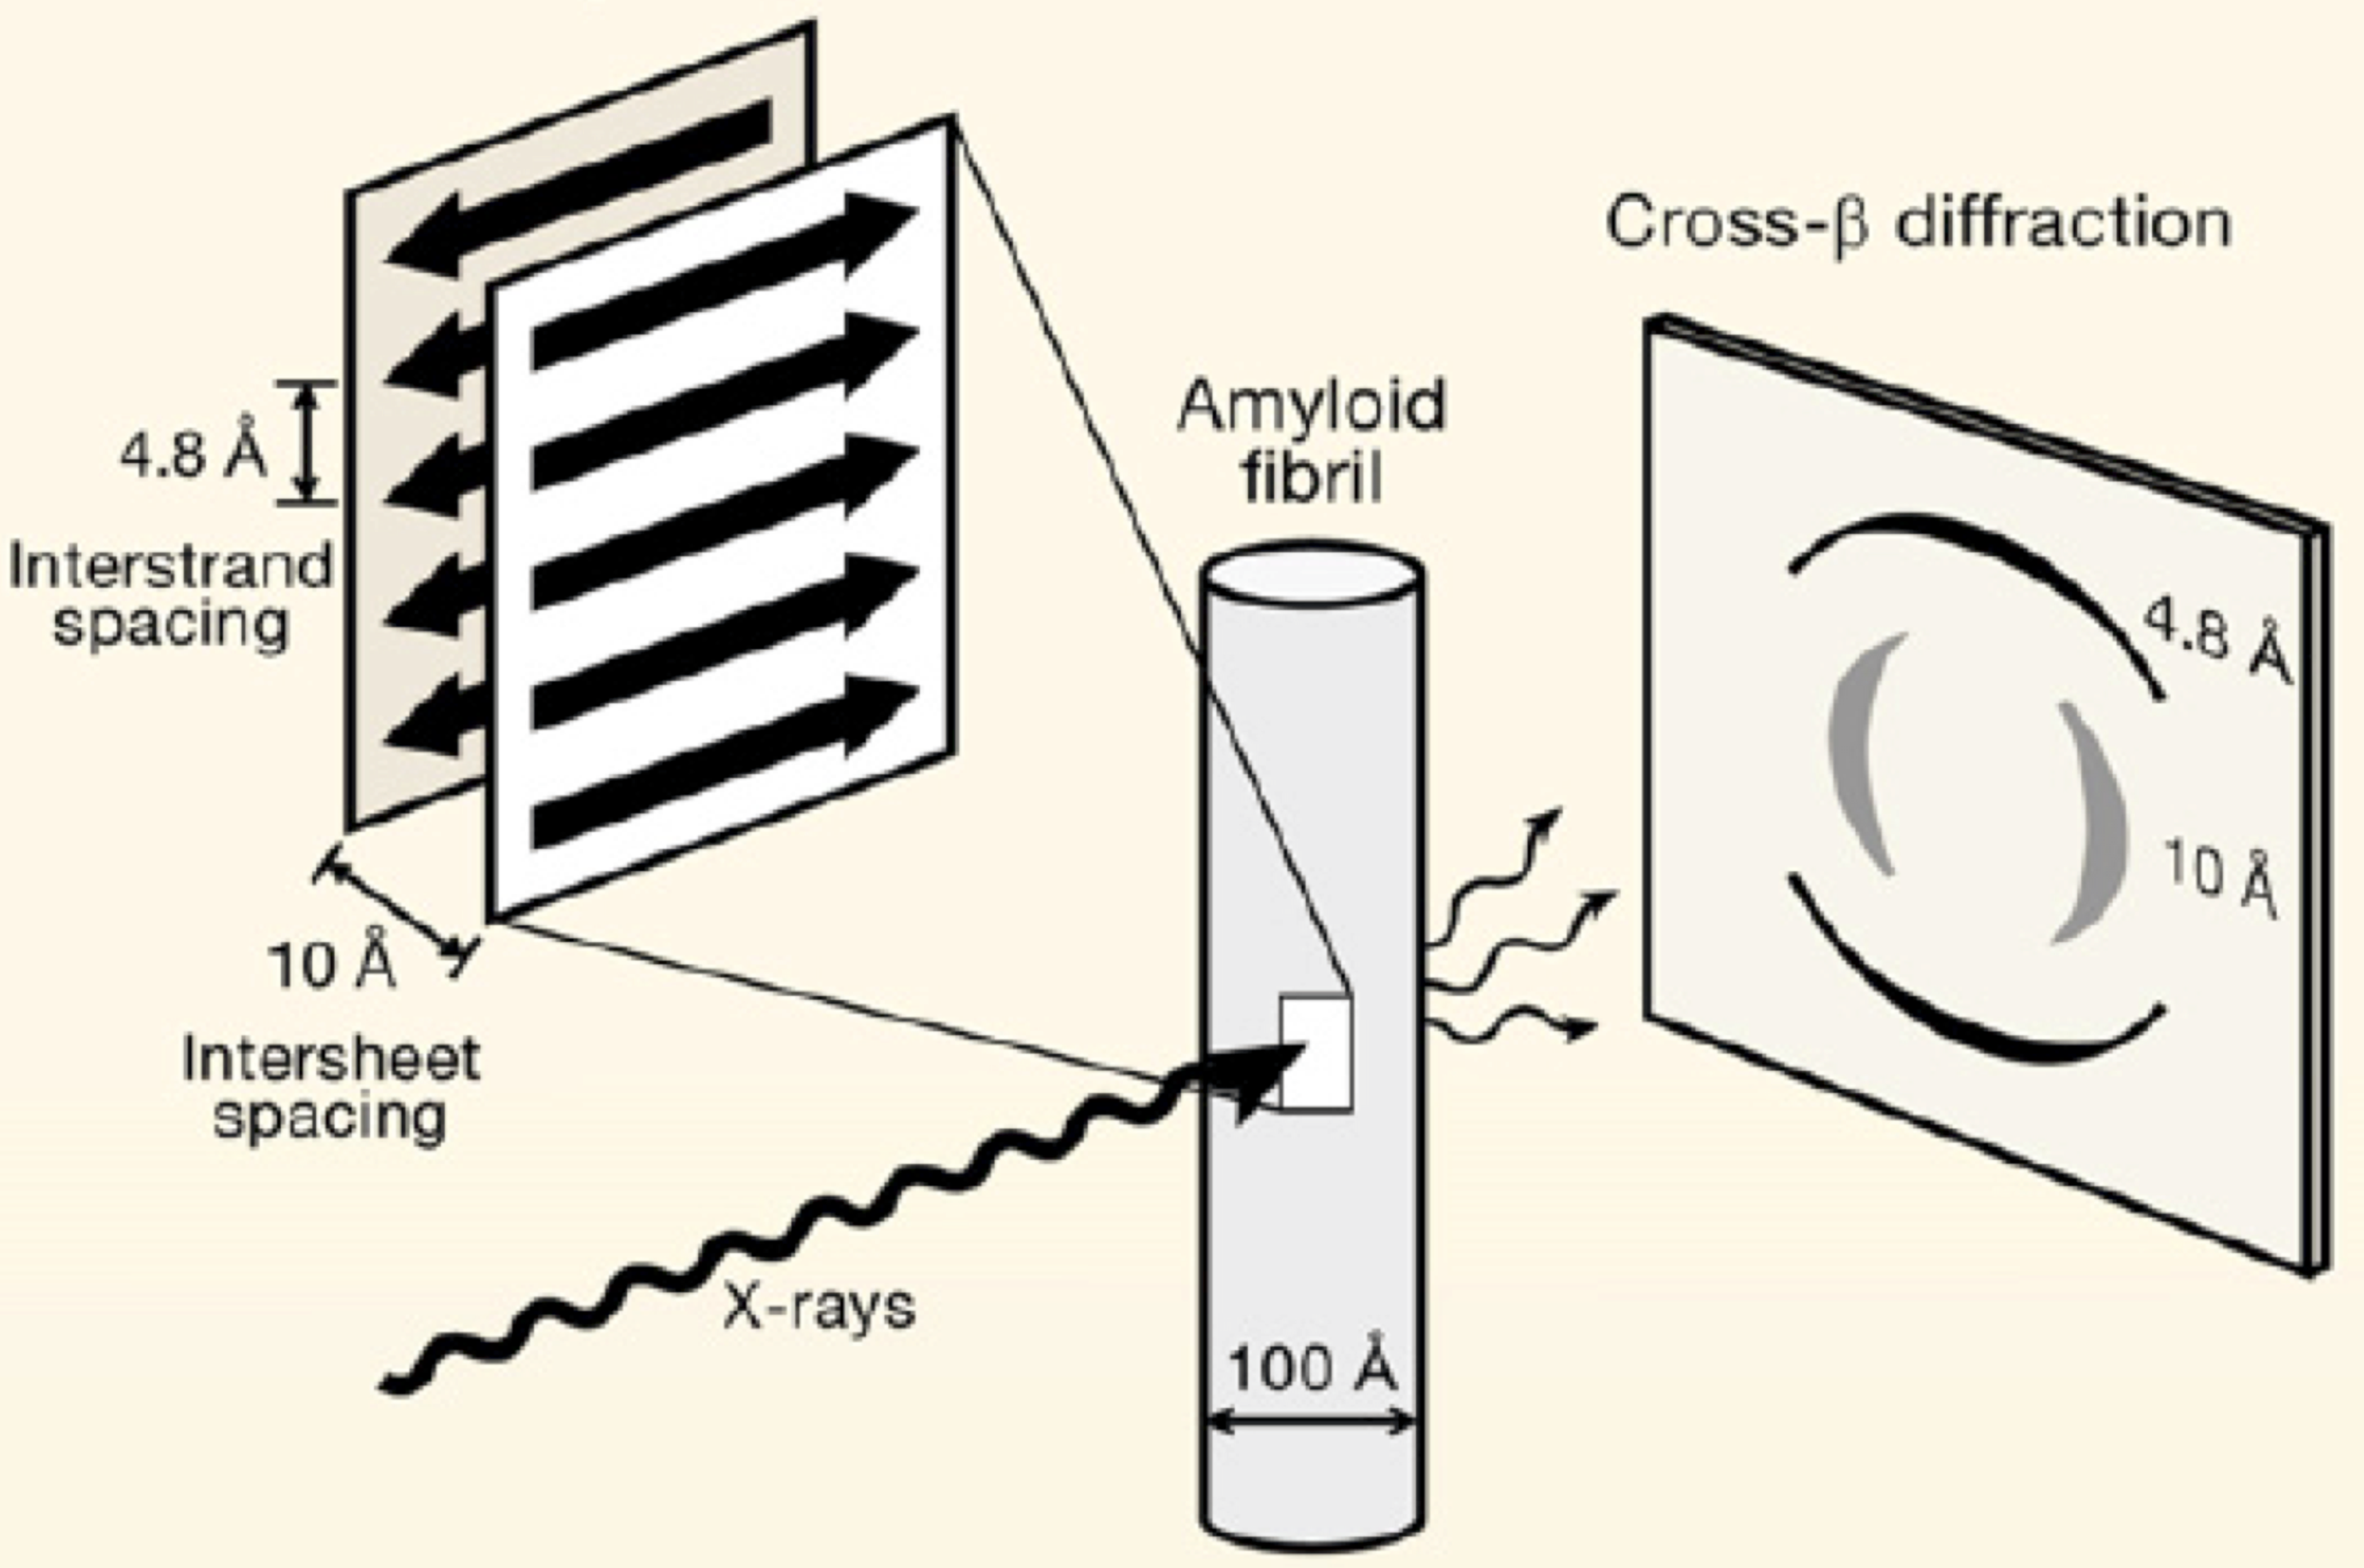
\includegraphics[width=6in]{figures/introduction/fibril_structure_diffraction.pdf}
  \caption[Characteristic cross-$\beta$ spacings from X-ray fibre diffraction studies of amyloid fibrils]{This is adapted from Eisenberg, 2012}
  \label{fig:fibril_diffraction}
\end{figure}

% Finding a treatment for AD and other fatal neurodegenerative diseases motivated many biochemical and biophysical studies of the amyloid state. 

Despite having dramatically different sequences, amyloid fibrils formed from different polypeptide all adopt a similar structure called the \crossbs.  The first structural studies of fibrils using X-ray fiber diffraction showed that a \crossb\ is characterized by a 4.8\angstrom\ interpeptide, and 10\angstrom\ intersheet spacing. XXX add more details to this description. XXX [Need to have a figure which shows this diffraction pattern, and EM data with cartoon model.] This defining characteristic of \crossb\ have now been adopted by biophysicists as an indication for the presence of amyloid fibrils.


Under the transmission electron microscope (TEM), fibrillar structures typical of many aggregates are visible as long, unbranched, often twisted ribbon-like structures nanometers in diameter (Figure~\ref{fig:fibril_TEM_SSNMR}). Independent measurements of fibrillar structure using different instruments have all confirmed the presence of \crossbs as the core structure of amyloid fibrils. (Figure~\ref{fig:fibril_diffraction})

% Other measurements 
% MPL Mass per unit length

Although \crossb\ is widely known, due to the insolubility and inherent non-crystalline nature of amyloid fibrils, the details of the fibril structure at the molecular level remained elusive until recently. Advances in solid-state NMR (SSNMR) and X-ray crystallography in the last decade have made major contributions to our knowledge of the molecular structure of amyloid fibrils.

\begin{figure}
  \centering
  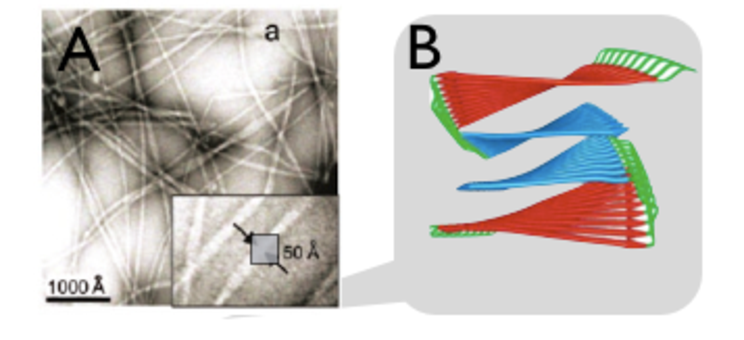
\includegraphics[width=6in]{figures/introduction/fibril_TEM_SSNMR.pdf}
  \caption[Characteristic cross-$\beta$ spacings from X-ray fibre diffraction studies of amyloid fibrils]{A Example EM images of oligomers.  Adapted from Bitan G. et al. 2003 and Walsh D. 1999 C TEM image of fibrils D SSNMR model proposed by Tycko et al.}
  \label{fig:fibril_TEM_SSNMR}
\end{figure}

% Describe the molecular structure of \abeta\ amyloid fibrils. 
% Briefly mention the techniques that can be used to obtain structural information of amyloid fibrils. 

% SSNMR
The initial molecular model of an amyloid fibril was for \abeta40, the peptide involved in Alzheimer's disease.  A SSNMR study on the amyloid fibrils of A$\beta$40 was done by Tycko et al in 2002. XXX The fibril core of \abeta40 involves the stretch sequence XXX-YYY. It is thought that residues A to B is disordered. The core fibril unit consists of a parallel in-register \bsheet, where each strand is a \bhairpin\ with peptide-peptide backbone hydrogen-bond along the long axis of the fibril. Figure~\ref{fig:fibril_TEM_SSNMR}


% X-ray structures
Furthermore, small peptide fragments that have characteristics of amyloid fibrils, which are also amenable to single crystal X-ray diffraction analysis have demonstrated similar type structures from those studied using SSNMR.  These structures obtained by X-ray crystallography have been described to have a dry interface with stacked sheets. (Figure~\ref{fig:fibril_xray_model})

\begin{figure}
  \centering
  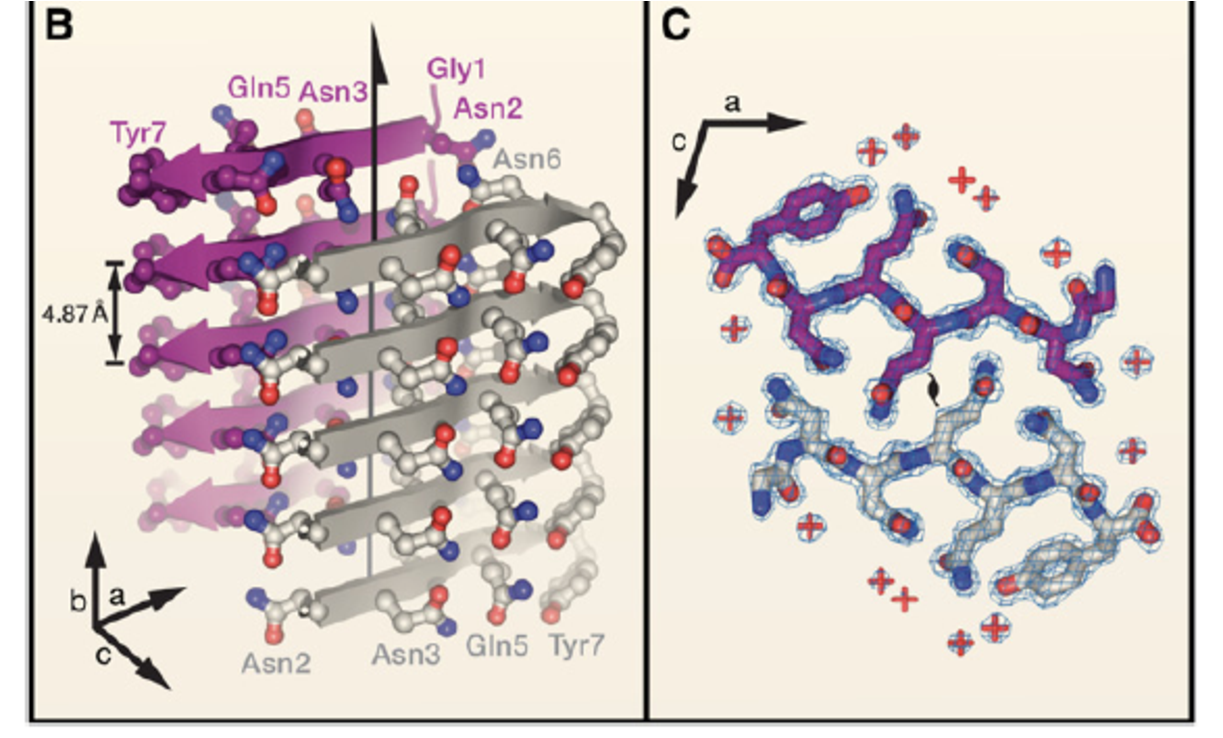
\includegraphics[width=6in]{figures/introduction/fibril_xray_model.pdf}
  \caption[Characteristic cross-$\beta$ spacings from X-ray fibre diffraction studies of amyloid fibrils]{This is adapted from Eisenberg, 2012}
  \label{fig:fibril_xray_model}
\end{figure}

% What do all fibrils have in common?
% Organization of the peptide backbone into beta-sheets; sheet stacking
The ubiquitous presence of a \crossbs supports that the organization of the peptidic backbone, common to all proteins, in to \bsheets\ is a major determinant of the fibrillar structure. Moreover, the proposed structures (some described above), indicate that the core region is composed of two to four sheets that interact closely with each other.

% I don't think I will talk about the twisting of the sheets too much.
% An interesting feature of these sheets is that they appear to be much less twisted than ex- pected from the analysis of the short arrays of β-strands that form β-sheets in globular protein structures. This feature was first proposed from cryo-EM and has been supported by Fourier transform infrared (FTIR) analy- ses (48, 61).

\subsection{Polymorphism of fibrils}

% Even fibrils formed from a single peptide can exhibit polymorphism .
Although all fibrils share the \crossbs, individual fibrils exhibit polymorphism at the molecular level which is dependent upon the experimental conditions under which they are formed.  % (Figure~\ref{fig:fibril_diffraction})
Fibrils may vary in the length of the beta-strand involved, side chain orientation. 

\subsection{Non-fibrillar oligomers}
\begin{figure}
  \centering
  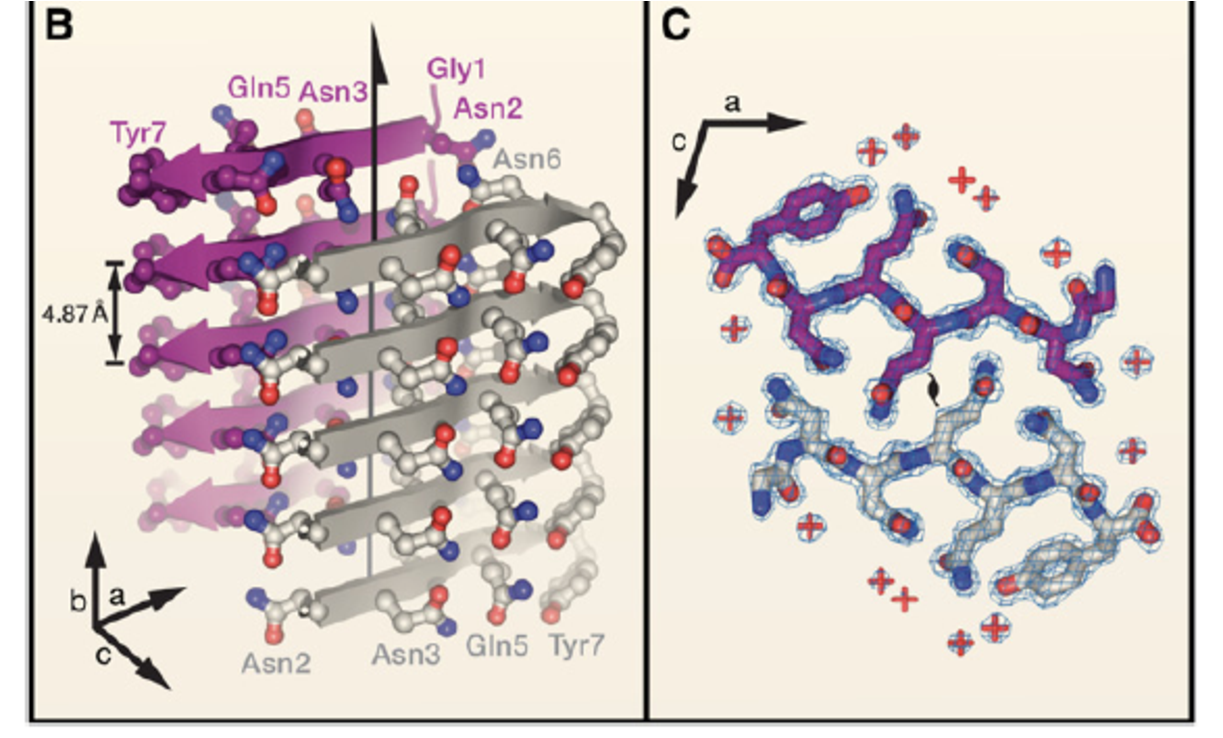
\includegraphics[width=6in]{figures/introduction/fibril_xray_model.pdf}
  \caption[Characteristic cross-$\beta$ spacings from X-ray fibre diffraction studies of amyloid fibrils]{This is adapted from Eisenberg, 2012}
  \label{fig:fibril_xray_model}
\end{figure}

Due to their structural disorder and their insolubility, molecular details of oligomers have been challenging to obtain using current structural determination techniques. 

EM and AFM experiments have shown that transient, unstable particles may appear prior to the formation of fibrils. In particular, soluble \abeta\ prefibrillar assemblies that are annular, spherical, or curvilinear in shape have been reported in literature.REF Protofibrils, in particular, are curvilinear, filamentous structures that are smaller than mature fibrils and are approximately 5-10 nm in diameter.9 Furthermore, protofibrils bind to dyes Thioflavin T (ThT) and Congo Red (CR), suggesting the presence of substantial β-sheet content.9, 13-15 Although some of these particles may be \bsheet-rich, they are morphologically distinct and are typically much smaller than fibrillar structures. Figure~\ref{fig:oligomers}

Despite the importance of these prefibrillar species in causing neurodegeneration, their molecular structures are still not known. However, a recent SSNMR study demonstrated that a late stage, neurotoxic Aβ40 spherical intermediate contained fibril-like β-sheet structure.16

[ Recent data show that non-fibrillar oligomers may contain fragments which are fibril-like in morphology. Most recently a study have shown that oligomers of \abeta\ ]
[ Should briefly read up on the book chapter by Pat Walsh]

\subsubsection{Amyloid Toxicity}
% I think outline some of the ideas / hypothesis about the link between amyloid and disease, but don't go into what people speculate or data on toxicity. It is related, but this is out of the scope of your thesis.

	% Key question in the field: What is the toxic species?
Multiple lines of research have identified oligomers as a likely causative agent for neuronal cell death. By contrast, the monomeric and fibril forms are thought to be less toxic than oligomers. It is hypothesized that soluble oligomers may cause toxicity by perturbing the integrity of cellular membranes through binding and disrupting the lipid bilayer (perhaps by making them ion permeable). \cite{Walsh:2007fu}

% Include a paragraph about amyloid formation and lipid membranes

% Understanding the toxicity or finding out whether there is a toxic species in part validates the amyloid hypothesis. 

% Here can lead into AD by saying well ... a widely known disease, where amyloid oligomers are thought to directly play a role in the disease process is AD.  

\section{Alzheimer's Disease}
One of the most well-known diseases involving amyloid formation is Alzheimer's Disease (AD), a devastating neurodegenerative disease that is most common cause of dementia in persons of age 65 or older.

% Pathological characterization
\begin{figure}
  \centering
  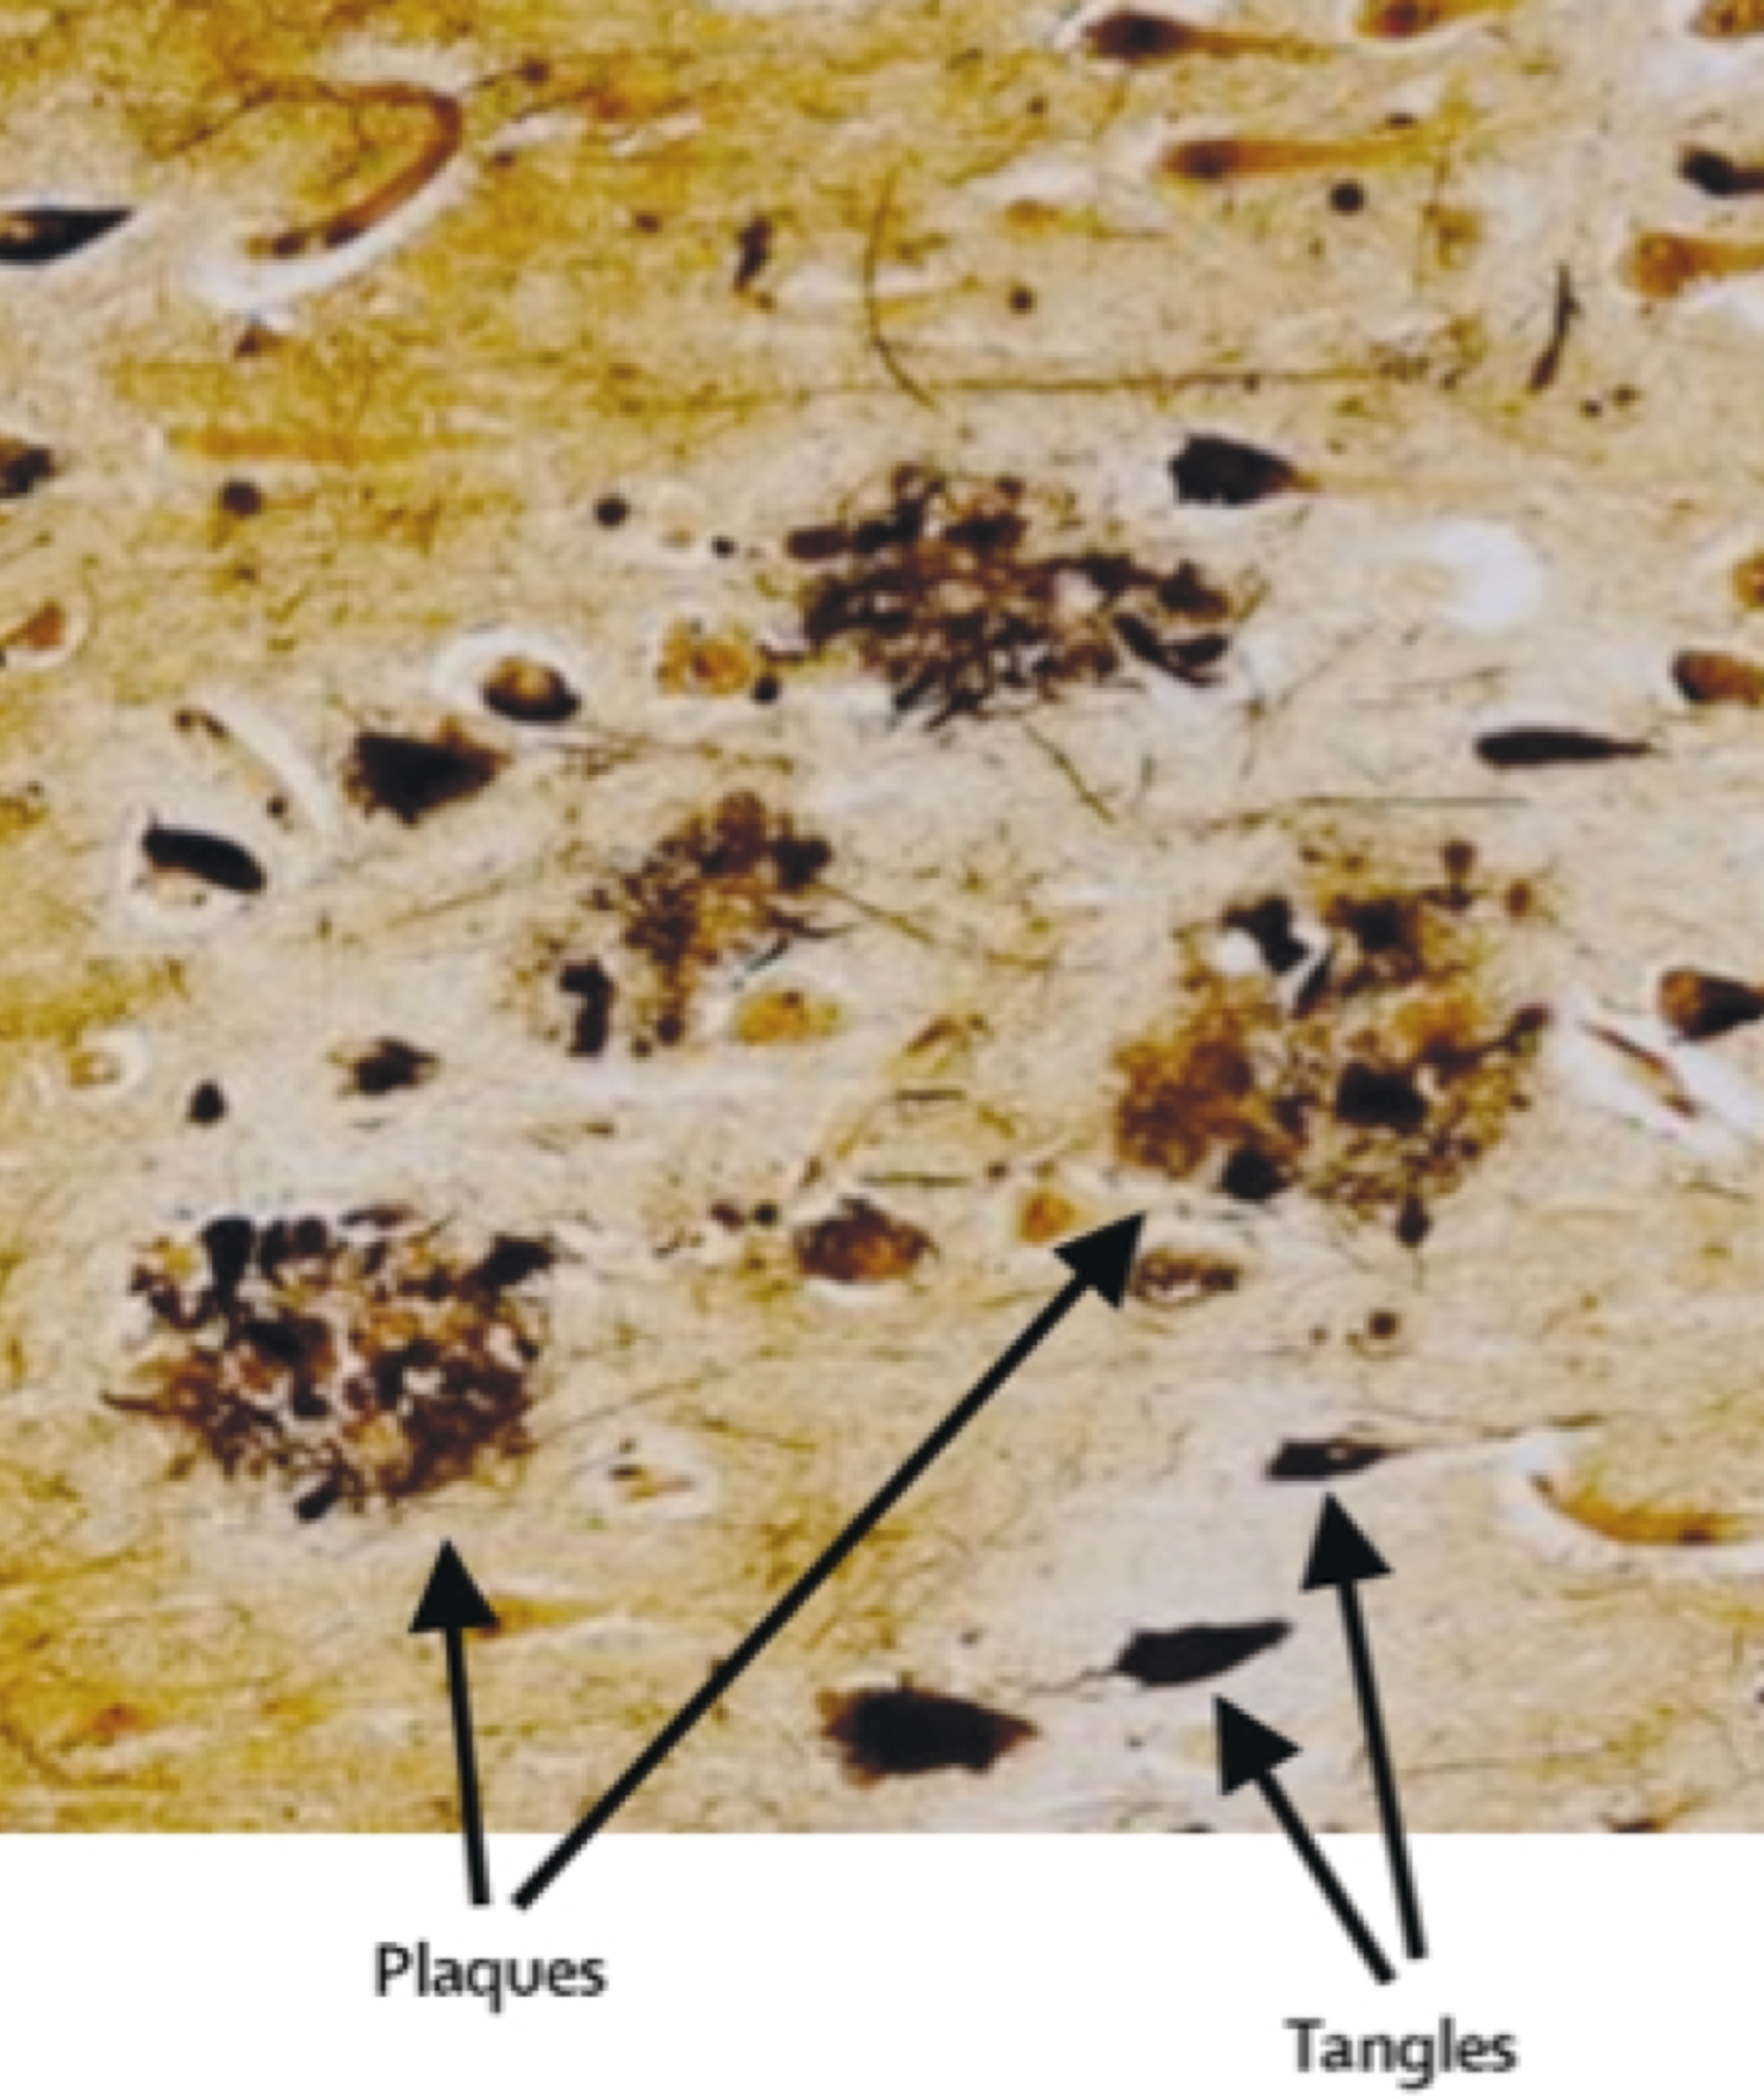
\includegraphics[width=6in]{figures/introduction/AD_tissue_pathology.pdf}
  \caption[Image of lesions formed by plaques and NFTs on brain tissue]{This is adapted from Blennow, 2006}
  \label{fig:AD_tissue_pathology}
\end{figure}

Upon examination, the brains of deceased AD patients show significant neuronal dystrophy.  Pathologically, AD is characterized by the presence of extracellular deposits of senile plaques and neurofibrillary tangles, which appear as lesions on stained neuronal tissue under light microscopy.(Figure~\ref{fig:AD_tissue_pathology})

Although it has been more than one hundred years since Dr. Alois Alzheimer first presented the association between the presence of neuronal plaques and the clinical symptoms of presenile dementia characteristic of Alzheimer's disease (AD), the exact relationship between the two is still under much contention.  It was not until in the 1980s, the protein \abeta\ was identified as the largest component of plaques. % How is Abeta produced ? Is it only involved in Abeta? What's the physiological role of Abeta?

The presence of amyloid plaque deposits in brains of deceased dementia patients led to the formulation of the long-standing amyloid hypothesis, which posits that amyloidogenesis of \abeta\ plays a key role in the initiation of AD. XXX

Although both plaques and NFTs appear together, many studies have indicated that NFTs plays a secondary role to \abeta\ in the pathogenesis of AD.
% More details on evidence which show that NFTs are not likely the causative species. Knock out mouse models ... mice do not develop AD, and instead develop tau pathologies  NFTs have also been shown to be affected by \abeta\ production.

% should I include more details on how Abeta is known to be produced in the body?
Monomeric \abeta\ is an approximately 4 kDa peptide produced by intramembrane proteolytic cleavage of the larger amyloid-$\beta$ precursor protein (APP) and is produced constitutively as part of the normal cellular metabolism.\{Selkoe, 2002 \#222\} APP is sequentially processed by the aspartyl proteases $\beta$-secretase and $\gamma$-secretase, where depending on the position of the cleavage by $\gamma$-secretase, a pool of \abeta peptides of lengths varying from 38 to 43 residues are produced. The peptides spanning residues 1-40 (\abetaforty) or 1-42 (\abetafortytwo) are predominantly found in AD-associated plaques. Neuritic plaques is composed of mainly \abetafortytwo, whereas \abetaforty\ is more commonly found in cerebralvascular plaques.

Multiple lines of evidence indicate that \abetafortytwo is likely to be the more deleterious form of \abeta. Genetic studies showed that mutations which cause early-onset AD also in turn increases the ratio of \abetafortytwo to \abetaforty.\cite{Hardy:1997tu} Moreover, in vitro, \abetafortytwo\ displays significantly higher propensity for aggregation than \abetaforty, despite differing by only two amino acids. In addition, \abetaforty\ and \abetafortytwo\ also have distinct aggregation pathways in vitro: \abetafortytwo is found to form a morphologically more diverse population of intermediate oligomers than \abetaforty.\cite{Bitan:2003ut}

% What about mice studies?

\abeta\ aggregates is present in a variety of morphologies in the brain. Although plaques are often visible in the dementia patients, the plaque load does not correlate with disease progression and severity, a puzzling aspect of AD.  Instead, synaptic loss correlated well with the concentration of soluble \abeta\ oligomers in the brain.

Currently there is a lack of treatment which targets the underlying disease. Most approved treatments today for AD only mitigates cognitive symptoms.  The vast number of structural and biochemical studies on amyloid structure have been crucial for the development of potential therapeutics for Alzheimer's disease.

%  Drug development for Alzheimer's has been on preventing amyloid aggregation and decreasing amyloid production. We will discuss this in more detail in later section XXX.
% Talk about how important it is to develop drugs for these amyloid disorders ... particularly for AD ... because it not only is a great economic burden on society, but a growing epidemic....

% \subsubsection{Other disorders}
% % Perhaps not enough to make it into its own subsection
% In addition to AD, other neurodegenerative diseases have been shown to involve the presence of amyloid.  Parkinson's disease, Huntington's, Prion disorders (Mad cow).  These diseases and their pathology are reviewed elsewhere and are beyond the scope of the thesis.
% I think I will not mention these things in detail in my introduction


\section{Amyloid Inhibition by small molecules: A promising method of treatment for AD}
% Cure, method of prevention; is there hope?

% In this section, I will provide an overview of some of the challenges to overcome when developing a small molecule therapeutic for Alzheimer's disease.  Furthermore, using this information, I will motivate why inositol is an exciting avenue to explore.

% Amyloid inhibition as a treatment for Alzheimer's disease and related amyloid disorders. 

% Briefly mention non-small molecule putative therapies which also acts via amyloid inhibition. The focus of this thesis will be on small-molecule amyloid inhibition.

% Use this as a transition into amyloid inhibition
% AD presents as a major economic and health burden to modern society.  With the longevity of our population, AD is approaching epidemic proportions with no cure or preventative therapy available.\cite{Blennow:2006wd}

Amyloids are attractive drug targets. Small molecules which targets amyloids may be an effective method of treatment for amyloid disorders because of the potential to treat the underlying disease. Through in vitro screening, many small molecules have been found to effect the amyloid aggregation pathway.  Some were demonstrated to inhibit amyloid fibrils, where as others were shown to arrest or reduce oligomer formation.
  
% Here I can take a cue from Justin Lemkul`'s recent review paper.
% Talk about the different kinds of small molecules that have been found to inhibition amyloid formation.  Here I will also provide a summary of what people know about the mechanism by which they inhibit amyloid formation.
Pharmacological perspective of the challenge of developing an Alzheimer's drug. In order to effectively treat Alzheimer's and other neurodegenerative diseases, small molecule drug candidates must pass the blood brain barrier at sufficient concentrations for inhibition.  This is difficult to achieve.
      
In vitro screening has led to the discovery of a large number of small-molecules which were found to affect the amyloid aggregation pathway. Many of these small molecules are thought to act by directly binding to amyloidogenic peptides and aggregates.

\begin{figure}
\centering
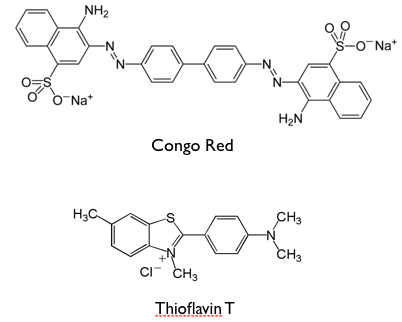
\includegraphics[width=3in]{figures/introduction/dyes.png}
\caption[Small molecule binders]{Amyloid binding dyes Congo Red and Thioflavin T}
\label{fig:amyloid_dyes}
\end{figure}

\subsection{Dye molecules}
Thioflavin T and Congo red are two dye molecules that are often used to identify the presence of amyloid fibrils.  

Early histological detection of amyloid binding was done using congo red, where upon binding fibrils exhibit red-green birefringence. Congo red requires the use of polarized light microscopy, a laborious process, and the interpretation of the birefringence is often not reproducible.

Thioflavin-T (ThT) is a benzathiole fluorescent dye also used to detect the presence of amyloid fibrils in post-mortem brain tissue samples, and monitor fibril formation in vitro. ThT exhibits a dramatic shift in the excitation spectrum maximum and an emission enhancement upon binding to fibrils, making it a sensitive and efficient report for the presence of amyloid fibrils.

Moreover, ThT is soluble in water and have \KD in the low \micromolar\ range.  ThT also binds uniformly across fibrils prepared from synthetic and biological sources.

The studies by Naiki et al. and LeVine showed that dye binding is linked to the presence of the \crossbs of fibrils, which led to the adoption of ThT dye binding as not only an indication of the presence of fibrils, but also as an indication of the presence of the \crossbs.

% Furthermore ThT fluorescence is only observed from those molecules that have bound to the fibrils.  
% ThT exhibits a shift in the excitation spectrum maximum, from 385 nm to 450 nm, and the emission maximum, from 445 nm to 482 nm

% This is from \cite{Wu:2011fd} which briefly summarizes why ThT binding gives rise to the excitation spectrum.
% These phenomena stem from two effects of binding.
% Firstly, steric and electronic stabilization (via charge trans- fer) of the ground-state charge distribution (7,8); and 2), restriction in the rotation of the aromatic rings of the dye (see Fig. 1 A) in its electronically excited state (9,10).



Both molecules appear to consistently bind mature amyloid fibrils.  Being \bsheet-rich does not imply that these dye molecules would bind. Also can affect fibril formation.(Fig.~\ref{fig:amyloid_dyes})

\begin{figure}
\centering
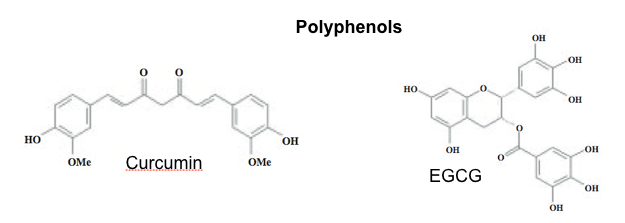
\includegraphics[width=6in]{figures/introduction/polyphenols.png}
\caption[Small molecule binders]{Polyphenols}
\label{fig:polyphenols}
\end{figure}

\subsection{Polyphenols}
Polyphenols,  is a large group of natural and synthetic molecules.  (−)-epigallocatechin-3-gallate, curcumin, and a polyphenolic grape seed extract, known for their anti-oxidant properties,  were recently discovered to be capable of affecting amyloid formation.(Fig.~\ref{fig:polyphenols})

\subsection{Inositol}
\begin{figure}
\centering
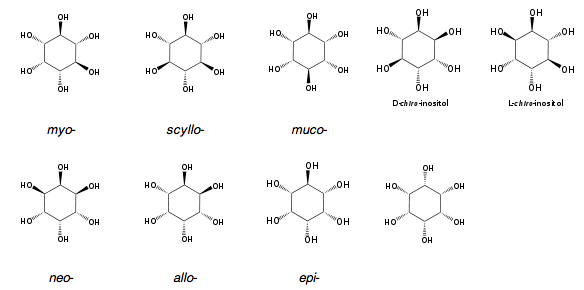
\includegraphics[width=6in]{figures/introduction/inositol.png}
\caption[Inositol]{Inositol stereoisomers}
\label{fig:inositols}
\end{figure}

% Should tell a little story of how inositol was discovered.  I remember that Chris Yip thought this might have been nice ... because it seems out of the blue to people.

% What I wrote in my transfer proposal:

Inositol with the molecular formula of \ce{C_6H_12O_6}, is a simple polyol with nine naturally occurring stereoisomers. Out of these nine isomers, seven are optically inactive, and the remaining two (L- and D-chiro-inositol) are chiral enantiomers.(Figure~\ref{fig:inositols})

% Here, use the physiological role of myo-inositol as a lead to transition into its role in amyloid inhibition.

Myo-inositol, the most abundant isomer, is ubiquitous in all eukaryotes and is a physiologically important osmolyte.  Furthermore, myo- is a precursor for inositol lipid synthesis: It is a constituent of phosphatidylinositol, an important phospholipid in membranes and second messenger systems. Once phosphorylated, myo-inositol phosphatides act as second messengers in intracellular signal transduction pathways.\cite{Fisher:2002tk}

Inositol is found in high concentrations in tissues of the human central nervous system (CNS): myo- And scyllo-inositol have approximate concentrations of 5 and 0.1-0.5 mM in the CNS, respectively.\cite{Fisher:2002tk} Accordingly, inositols also function as osmolytes in the CNS, where alterations in their concentrations are known to be associated with neuropathological conditions.\cite{Michaelis:1993gf, Fisher:2002tk}

% Role of inositol in amyloid inhibition. Here, include the background on how inositol was discovered as an \abeta\ amyloid fibril inhibitor
In recent years, scyllo-inositol have been identified as a promising therapeutic candidate for the treatment of Alzheimer's Disease.

Scyllo-, myo-, and epi-, but not chiro-inositol, have been shown to inhibit \abeta42 fibril assembly, stabilize an oligomeric complex of \abeta42, and attenuate \abeta-oligomer-induced neurotoxicity in vitro. Moreover, inositol exhibits stereochemistry-specific effects on \abeta\  fibril inhibition and cytotoxicity: scyllo- and epi- are more effective than myo-inositol, whereas chiro-inositol was inactive.\cite{McLaurin:2000bq}

An important therapeutic advantage of scyllo-inositol is its ability to readily crosses the bloodbrain barrier (BBB) (both actively and passively transported). Because it is not enzymatically broken down in the gut, it may be administered as a drug orally. 
% Inositol is synthesized inside the body ... or can be obtained via nutrition?  
		
In vivo studies with a transgenic mouse model of AD demonstrated that alleviation of symptoms after inositol treatment was correlated with a decrease in the levels of soluble \abeta\ oligomers, suggesting that the beneficial effects of scyllo-inositol may be attributed to the inhibition and/or disaggregation of high-order \abeta\ oligomers.\cite{McLaurin:2006eb}

Taken together, these results suggest that scyllo-inositol, and its derivatives, are a potential therapy for AD with the ability to change the course of the disease.\cite{Nitz:2008jl,Sun:2008ko}

% Include some data on human clinical trials (?) -- II was negative ... how to say it ? Should read phase II paper.
Presently scyllo-inositol completed both phase I and II of human clinical trials, where it was demonstrated that inositol is not toxic to healthy individuals at concentrations effective for amyloid inhibition.

\subsection{Commonalities between small molecule inhibitors}
% Commonalities between small molecules which appear to affect amyloid aggregation
Small molecule inhibitors share common chemical features and groups.  They are typically planar in geometry, have many aromatic rings, and polar functional groups (hydroxyl groups) around the edge of these aromatic rings.



\subsection{Molecular mechanisms of amyloid inhibition 
	            \\ by small molecules}
% Mechanism of action.
Some small molecules inhibit fibril formation, where as others may prevent oligomerization, but not fibrillation. A high concentration is often required to observe activity (micromolar to millimolar), which suggests that they may be non-specific inhibitors. EGCG, one such polyphenol, is known to have the lowest IC50.
    	% IC50 -- This quantitative measure indicates how much of a particular drug or other substance (inhibitor) is needed to inhibit a given biological process (or component of a process, i.e. an enzyme, cell, cell receptor or microorganism) by half.
      % EC50 -- The term half maximal effective concentration (EC50) refers to the concentration of a drug, antibody or toxicant which induces a response halfway between the baseline and maximum after some specified exposure time.[1] It is commonly used as a measure of drug's potency.
      % Ref: wikipedia
      
  	% Review of what is known about amyloid fibril ligand binding, specifically dyes.

Molecular mechanism of binding of dye molecules. Thought to bind flat on on the surface grooves of amyloid fibrils where they interact with hydrophobic groups exposed at the surface. 
      % Doesn't explain why the dye molecules are also able to suppress fibril formation.
      % Can the birefringence be explained by these binding modes? -- this is out of the scope of my thesis.  Don't put this in my thesis but I should be able to coherently explain this during my defense.

\section{Analogy to Sugar-protein binding}
% Does this section fit here? Where should I put it?
% Could use this as a prime example of protein-ligand interaction ...
% As a prime example of protein ligand interaction, one of the first systems that was used to understand binding was a sugar binding protein lysozyme ... -- No I think I will use early systems used to understand protein-ligand binding and if that was a sugar binding protein, then it will come off as a coincidence.
% This section is best discussed in the context of understanding inositol binding ...

% Mention some experimental techniques used to obtain protein sugar-binding modes, but the point here is not to review these methods ... but to point out that I am aware of these techniques.

\subsection{Sugar Binding modes}

% This section provides a nice lead in to the methods section
\section{Protein-ligand interactions}
\subsection{Forces involved in binding}
% Note that I may end up introducing the forces up in the earlier section -- reorganize as needed
\begin{outline}
	\1 Protein-ligand non-covalent interactions that are important for ligand binding and recognition
		\2 Electrostatic interactions. Polar (hydrogen bonding) and charge-charge interactions
		 % Here, it will benefit me to read Sarah's appendix C carefully.
		\2 Nonpolar (hydrophobic) interactions
		  \3 Van der Waals
\end{outline}

\subsection{Binding equilibria}
% subsection protein_ligand_binding_theory (end)
% Below is a summary of an excerpt from Tom's thesis on structure-based drug discovery.
% Design of antibiotics 
% 1) Target determination (biochemical)
% 2) Structural determination (Xray, NMR, or homology); active site identified; Here would be useful to get the holo structure of the protein
% 3) Screen for inhibitors against a chemical library or in silico docking.
\begin{outline}
	\1 Enzyme and its putative ligand typically bind specifically (high affinity binding).  We want to optimize binding specificity to increase the efficacy of the putative drug, and decrease adverse side effects (toxicity) in the human body.

	\1 The dissociation constant, $K_d$, is a measure of the affinity of a ligand for its binding site on the host protein. Pharmacologically, it can be interpreted as the concentration at which 50\% of the drug is bound to the protein. In experimental studies, $K_d$ is often used to quantitatively screen for potential drug candidates. 
  % A small $K_d$ suggests that the ligand may bind tightly to the protein.

	\1 Binding equilibrium

    \begin{equation}
      \left[ Protein\cdot Inositol \right] 
      \rightleftharpoons 
      \left[ Protein \right]+\left[ Inositol \right]
    \end{equation}
  
    % \2 Absolute binding free energy
    % \2 Relative binding free energy
    
	\1 The binding free energy of a ligand to a protein is directly related to its dissociation constant, $K_d$, the equilibrium constant of the above reaction

     \begin{equation}
        K_{d} = f_{ub}\frac{\left[ Protein \right]\left[ Inositol \right]}{\left[Protein \cdot Inositol\right]},
     \end{equation}
     
     % Add equation converting binding constant to gibbs free energies.
	\1 Experimental techniques for estimating $K_d$
		\2 What experimental techniques are used to estimate binding affinity? (May need to study up on this)
		\2 Isothermal titration calorimetry (ITC) is a technique which can be used to measure energetics of ligand binding to peptides.
\end{outline}

% \subsection{Role of chirality in drug binding}
% Stereoisomerism is important to the activity of molecules.  It modulates binding to proteins.
% Two types of stereochemistry
% Constitutional isomers - differs in bonding sequences and connectivity
% Stereoisomers - differs in orientation of their atoms in space, but no connectivity differences.
% Definition of chirality [Add schematic] ... etc
% Molecules with chirality have a non-superimposable mirror image, called an enantiomer.
% A carbon molecule with four different groups has chirality.

\section{Thesis objectives and rationale}
% Understanding amyloid inhibition in the context of the framework of traditional enzyme inhibition mechanism
\subsection{Challenges of amyloid inhibition}
\begin{outline}
       % However, most of these studies were focused on A$\beta$ and large A$\beta$ aggregates,\{Fawzi, 2008 \#553;Esposito, 2008 \#567;Sgourakis, 2007 \#609;Wei, 2006 \#656;Tarus, 2006 \#628 Karsai, 2006 \#658\} and thus, were computationally limited by the complexity of the molecular systems.

    \1 The protein-ligand binding model developed to understand enzyme inhibition cannot be directly applied to understand the molecular mechanism of amyloid inhibition by small molecules. 
    
      \2 Amyloid inhibitors are found to be very weak binders. How do non-specific inhibitors act as a drug? And how do we approach this with MD simulations?
      
      \2  Because the A$\beta$ amyloid aggregate pathway encompasses a variety of species, some of which has no folded structure, a single conformation cannot be assumed for binding. Furthermore, structural information of amyloidogenic species lags behind those of enzymes, which tends to be globular proteins amenable for X-ray crystallography. This means that the putative binding sites are not known.
      
      \2 The structural disorder of the peptides involved poses a challenge for obtaining converged properties from MD simulations. 
    
    	\1 A$\beta$ peptides are completely disordered.  We also do not know what the binding site looks like, where it is located on these structures.
    	
    \1 To date, few studies have attempted to provide statistically meaningful results pertaining to general mechanisms of protein self-aggregation and amyloid formation. Furthermore, despite the abundance of MD studies of A$\beta$, few studies have systematically examined the mechanism of action of small molecule inhibitors of amyloids

    \1 In AD, there is the added challenge of the drug being able to cross the brain barrier, while remaining non-neurotoxic.  What kind of drugs cross the BBB?  Typically hydrophobic drugs.
\end{outline}    

\subsection{Study Design and Rationale}
\begin{outline}
	\1 Here describe in detail how I designed my study to circumvent the challenges presented by the amyloid inhibition problem, and the limitations  of MD simulations. At this point, clearly explain and discuss my study design and rationale. (Fig.~\ref{fig:rationale})

  \begin{figure}
    \centering
    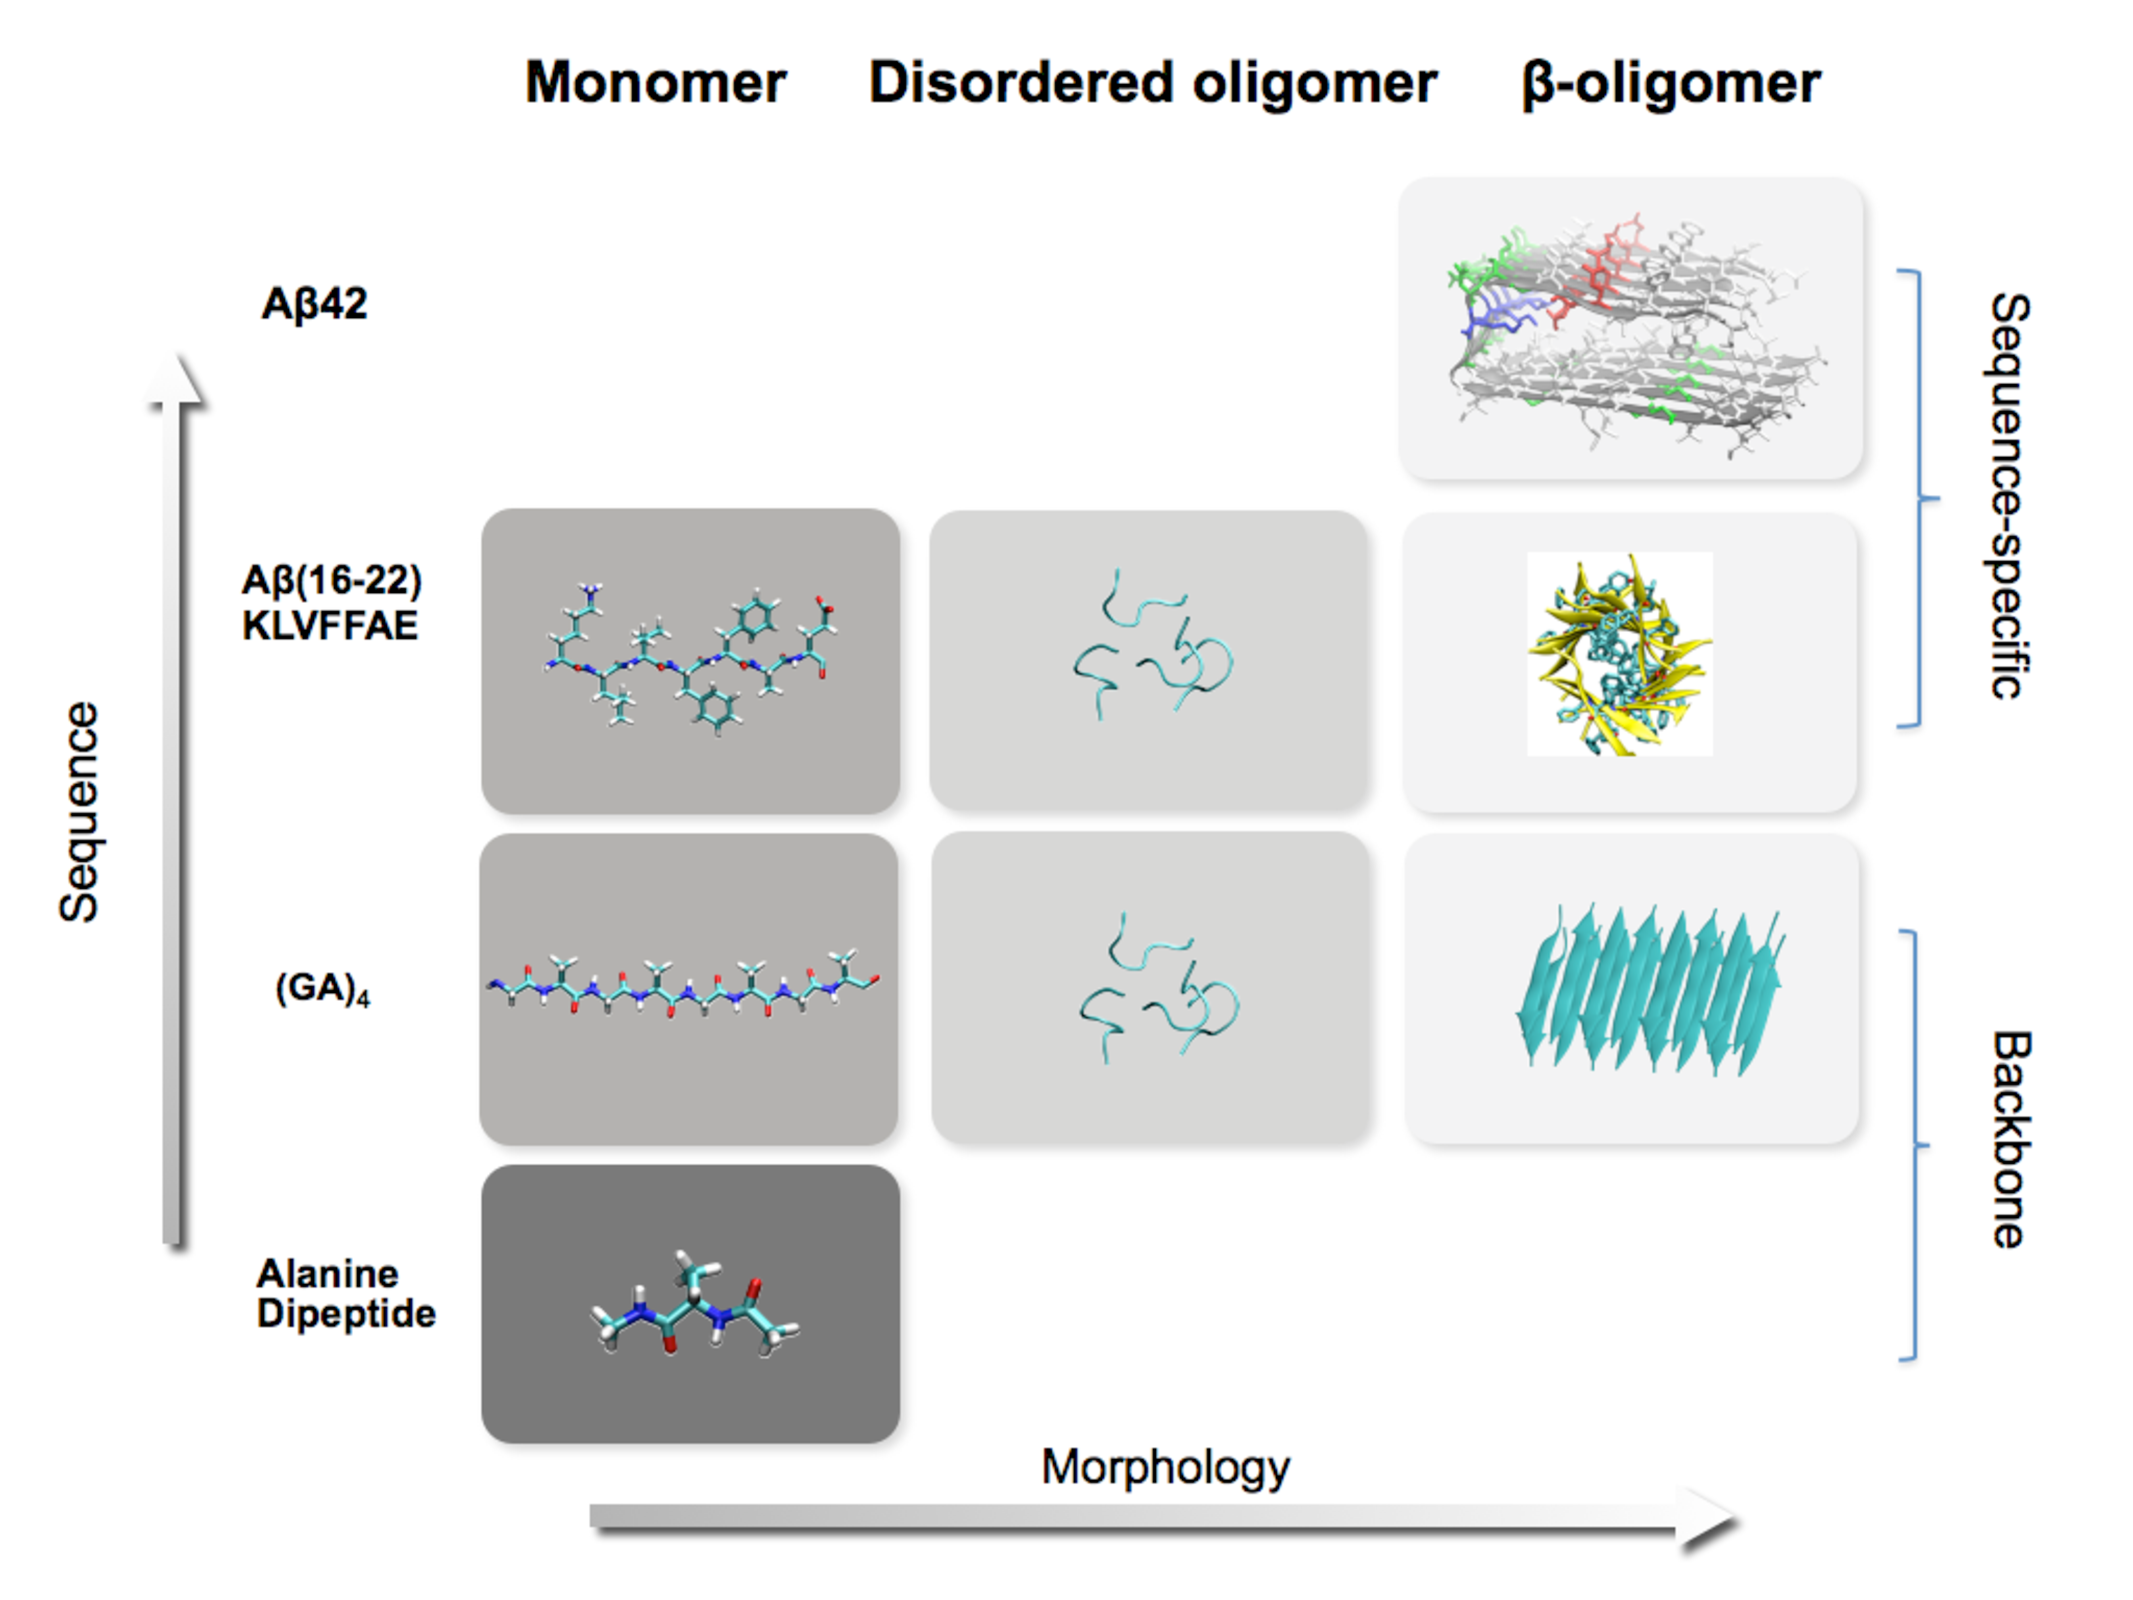
\includegraphics[width=6in]{figures/introduction/matrix.pdf}
    \caption[Rationale]{Shows the progression from small, model systems to larger and structurally more complex systems involving the full-length A$\beta$42 peptide.}
    \label{fig:rationale}
  \end{figure}

	\1 Beginning with the simplest model systems for an amyloidogenic peptide, the alanine dipeptide, we systematically examine binding of inositol with systems of both increasing sequence and structural complexity.

	% Use brute force simulations
	\1 We exploit conventional MD simulation techniques because simulation approaches used for understanding enzyme-ligand binding is not applicable. 
	
	\1 Instead, we use conventional MD simulations and repeats of independent simulations to determine the binding modes, and binding equilibria of inositol with amyloidogenic peptides and aggregates of A$\beta$.
\end{outline}

\section{Thesis Organization}
The first chapter introduces the thesis in the context of the field.  The second chapter introduces the main methods used in the work in the thesis. Chapters 3, 4, and 5 are the results of simulations of inositol with amyloid like peptides and aggregates. Chapter 6 shows work of the general applicability of our methods developed throughout this thesis to MD simulations to understand protein - carbohydrate binding. Chapter 7 provides discussion, suggestions for future work, and perspectives.

\addcontentsline{toc}{section}{Bibliography}
\bibliographystyle{plain}
\bibliography{chapter1}

% AD
% Treatment - harder to treat - lack of biochemical understanding of what causes disease, which makes it difficult to develop drugs for; lack of good diagnostic methods because treatment may not be effective at end stages of the disease where brain function won't e able to be rescued.
% Diagnosis - hard to diagnose
% AD is difficult to diagnose.  It is often not apparent that someone has AD until they exhibit symptoms severe enough to interfere with daily life or occupation. 

% Amyloid hypothesis - our best guess at what causes AD and provides the best guess at what we should be targeting. 
% Abeta Amyloid thus far provides the best clue to the molecular basis of AD, and thus a promising pathway to a cure for AD.

% In some individuals without dementia symptoms may have as much plaque as another with severe AD. Synaptic loss can be used as a measure of disease progression. 

% Perhaps use this as a transition into the general discussion of amyloid formation and structure -- not only specific to Abeta.
% Furthermore, amyloid have also been known to play beneficial roles in certain living systems. REF
% Increasing awareness of the amyloid state of proteins, and interest grew in amyloids because of their role in a variety of devastating human diseases.

% Fibrils

% In this section I will talk about how amyloid aggregation is thought to work. Introduce the thermodynamic model for understanding fibril formation.
\chapter{Introduction (outline)}
\section{notes}
% agonist:  a molecule that binds to and "actives"


\subsection{Alzheimer's Disease}
\begin{outline}
\1 Alzheimer's was discovered nearly a hundred years ago and yet still does not have a cure today.  Alois Alzheimer met a women in her 60s that did not know herself. Now it is known that Alzheimer's Disease (AD) is a progressive neurodegenerative disease and is the most common form of dementia in persons of age 65 or older. With the increasing longevity of our population, AD is approaching epidemic proportions with no cures or preventative therapy available.\{Blennow,2006 \#221\}

\1 Years later A$\beta$ was produced synthetically in the lab. A$\beta$ was found to clump together and precipitate out of solution almost immediately, which led to the discovery of amyloid fibrils.

\1 AD was the main motivator for amyloid science. The study of amyloid as being spun out of many years studying AD.

\1 A long-standing hypothesis known as the amyloid hypothesis states that amyloid is the underlying cause of the pathogenesis of Alzheimer's disease.  Amyloid is thought to be toxic species.  It is most recently hypothesized that amyloid causes cellular toxicity by perturbing the cell membrane (making them ion-permeable).
\end{outline}

\section{Amyloid}
\begin{outline}
\1 Amyloid aggregation pathway. Monomers aggregate to form oligomers. There are different type of oligomers. Some are on-pathway to fibril formation. Some are found to be end-points of the aggregation pathway. 

\1 Aggregates are implicated in disease toxicity.  The structure of these aggregates have been difficult to obtain via traditional experimental protein structural determination methods because many of the aggregates aren't soluble and are structurally disordered.
\end{outline}
    
\section{Amyloid inhibition by small molecule binders}
  \begin{outline}[enumerate]
    \1 Amyloids are a attractive drug target.  Many small molecules are found to bind to amyloids and inhibit amyloid fibrils.   Small molecules may be one effective way to develop a treatment for amyloid disorders because they have the potential to be developed into drugs.
    
    \1 In order to effectively treat Alzheimer's, requires small molecule to pass the blood brain barrier.  This is a difficult thing to achieve. 
    
    \1 Some small molecules inhibit fibril formation, some inhibits oligomerization. They are all found to be weak binders and act on millimolar concentrations. The strongest activity is EGCG

    \1 Thioflavin T and Congo red are dye molecules which are used in identifying the presence of amyloid.  Both molecules bind to the fibrillar form of amyloids.

    \1 Another class of molecules which binds to one or species of amyloid is polyphenols such as EGCG. These molecule is found in green tea and wine.
  
    \1 These molecules are found to be weak binders.  That is, they bind at high concentrations.  
  
    \1 They share common chemical features.  All of them are planar in geometry, have aromatic rings, and polar functional groups around the edge of these aromatic rings.
  \end{outline}

\section{Molecular simulations}
% Why MD?
% To properly understand drug binding - we need motion!

% The first thing that want to talk about is why people have used molecular dynamics to study proteins.  Think about the reader ... they should not have questions like ... why can't you just use docking, pick a single structure -- no single structure.  Can't assume binding sites!  

% Why couldn't you have just taken A$\beta$42 and simulated that from the beginning, why model peptides?  Because computationally infeasible?  -- Why ?  I think the answer comes down to answering in part why computing protein folding is hard.

% Is MD is just pretty pictures or can we get quantities that are experimentally comparable.  Are some of these things experimentally testible?  -- what are some things that I've tried to compute in my simulations that others haven't been able to do? This will be something that I should anticipate and be ready to address at my defense.  In sum, all the stuff that ever came up at my student seminar and my committee meetings ... I should be ready to answer.


Examples are to study protein dynamics - importance of protein dynamics

What is molecular dynamics simulations. A set of numerical computation algorithm which solves numerically solves the N-body problem. Solves a system of Newton's equations of motion, and provides the time-trajectory of atoms with femtosecond time resolution. The integration algorithm is XXX. Time steps used are typically 2 femtoseconds to capture the hydrogen bond vibrational motion. [MORE DETAILS AND EQUATIONS HERE]

Step to produce a molecular simulation:
First take a structure from crystallography or NMR, or homology-modelling data.
In the algorithm, the forces acting on each atom are estimated from [insert equation here]

[Ref: Chris Madill's and Tom's thesis]


\subsection{Determining protein-ligand binding free energies}
Have an X-ray crystal structure and know of a putative binding pocket. [See Tom's thesis]
Ligands typically have high binding affinity to a binding pocket. Here, we want to  Binding is a low probability event and therefore infeasible to simulate using brute-force MD sampling.

\subsection{Application of MD simulations to amyloid inhibition}
MD studies using brute-force sampling.

Aid in medicinal chemistry by making suggestions for how to design new AD drugs

% Model peptides
% Chapter cover page
\chapter{Binding of inositol stereoisomers to model amyloidogenic peptides}

The contents of this section were adapted from an article published in the \emph{Journal of Physical Chemistry}.
\\
\\
\emph{Reference}:
Li, G., Rauscher, S., Baud, S., & Pomès, R. (2012). Binding of Inositol Stereoisomers To Model Amyloidogenic Peptides. Journal of Physical Chemistry B, 116(3), 1111–1119.
\\
\\
\emph{Contributions}:
Grace Li conducted the research and wrote the section. Régis Pomès provided editorial input and guidance.

\newpage

\section{Summary}
The self-aggregation of proteins into amyloid fibrils is a pathological hallmark of numerous incurable diseases such as Alzheimer's disease. Scyllo-inositol is a stereochemistry-dependent in vitro inhibitor of amyloid formation. As the first step to elucidate its mechanism of action, we present molecular dynamics simulations of scyllo-inositol and its inactive stereoisomer, chiro-inositol, with simple peptide models, alanine dipeptide (ADP) and $(Gly-Ala)_4$. We characterize molecular interactions and compute equilibrium binding constants between inositol and ADP as well as, successively, monomers, amorphous aggregates, and fibril-like β-sheet aggregates of $(Gly-Ala)_4$.\cite{Balbach:2000p49}

Inositol interacts weakly with all peptide systems considered, with mM to M affinities, and displaces the conformational equilibria of ADP but not of the $(Gly-Ala)_4$ systems. However, scyllo- and chiro-inositol adopt different binding modes on the surface of β-sheet aggregates. These results suggest that inositol does not inhibit amyloid formation by breaking up preformed aggregates, but rather by binding to the surface of pre-fibrillar aggregates.

\section{Introduction}
Amyloid fibrils formed by various peptides and proteins are known to be associated with neurodegenerative diseases, type II diabetes, and prion-related disorders.{Chiti, 2006 #101} In particular, amyloid fibrils of Aβ peptides are found in the extracellular deposits of neuronal plaques and are thought to be central to the pathogenesis of Alzheimer’s Disease (AD),{Chiti, 2006 #101;Hardy, 2002 #76} a common and incurable neurodegenerative disease causing dementia and eventual death. 

In recent years, amyloid fibril formation was discovered to be a common phenomenon among many proteins in vitro; that is, under certain misfolding and denaturing conditions, proteins can self-aggregate to form amyloid fibrils.{Chiti, 2006 #101} When viewed with negatively-stained transmission electron microscopy, amyloid fibrils appear as elongated, rope-like structures that are often 100 nm in length.{Chiti, 2006 #101} The core structure of all amyloid fibrils is the cross-β sheet.{Chiti, 2006 #101;Serpell, 2000 #88} At the molecular level, NMR{Balbach, 2000 #95;Petkova, 2006 #109} and X-ray crystallography{Sawaya, 2007 #103} studies have revealed that the cross-β structure is comprised of extended polypeptides organized in highly-ordered, in-register β-sheets. Although amyloid fibrils are a pathological hallmark of amyloid-based diseases, smaller nonfibrillar oligomers as little as three or four peptides in size have been demonstrated to display higher cytoxicity than mature fibrils.{Gong, 2003 #122;Bitan, 2003 #81;Kitamura, 2010 #107;Keshet, 2010 #124;Selkoe, 2008 #116;Lambert, 1998 #106;Caughey, 2009 #110}

An important strategy to finding a cure to AD and other amyloid diseases is to derive new therapeutic candidates through the rational design of effective small-molecule inhibitors of amyloid formation. In recent years, a number of small molecules capable of preventing aggregation and/or fibril formation have been discovered and have emerged as potential therapeutic approaches for protein misfolding diseases.{Necula, 2007 #113;Hawkes, 2009 #108;Frid, 2007 #98;LeVine, 2009 #79;Scherzer-Attali, 2010 #121;Sood, 2009 #65} Interestingly, many of these small molecules share common chemical structural features, such as aromaticity and the presence of multiple hydrogen-bonding groups.{Porat, 2006 #67;Ehrnhoefer, 2008 #85;Liu, 2009 #105;Liu, 2005 #117} However, the molecular basis of the structure-activity relationship of these small molecules is not understood, thus hindering drug development efforts for amyloid-based diseases. 
Recently, one such small molecule, scyllo-inositol, has shown promise as a therapeutic for AD.{McLaurin, 2000 #70;McLaurin, 2006 #115} Scyllo-inositol is one of nine stereoisomers that belongs to a class of cyclic polyols called cyclohexanehexols. Four stereoisomers, myo-, epi-, scyllo- and chiro-inositol (Fig. 1) are physiologically active.{Fisher, 2002 #90} Myo-inositol, the most abundant stereoisomer, plays an important role in signal transduction as precursor of phospholipid headgroups: once phosphorylated, myo-inositol phosphatides act as second messengers in intracellular signal transduction pathways.{Fisher, 2002 #90} Importantly for its therapeutic potential, inositol readily crosses the blood-brain barrier. Myo- and scyllo-inositol are found in tissues of the human central nervous system (CNS), with approximate concentrations of 5 mM and 0.1 to 0.5 mM, respectively.{Michaelis, 1993 #135} Accordingly, they are also important osmolytes in the CNS, where alterations in their concentration have been associated with neuropathological conditions.{Fisher, 2002 #90;Michell, 2008 #73}

In vitro, inositol stereoisomers stabilize nonfibrillar β-structure and prevent the formation of amyloid fibrils in a stereochemistry-dependent manner: scyllo-, epi- and myo-inositol inhibit Aβ fibril formation, but not chiro-inositol.{McLaurin, 1998 #129;McLaurin, 2000 #70;Nitz, 2008 #71;Sun, 2008 #96;Townsend, 2006 #91} Moreover, scyllo-inositol was also demonstrated to be the most effective stereosiomer in preventing and reversing AD-like symptoms in transgenic mice while reducing their brain plaque load.{McLaurin, 2006 #115} Despite this progress, the molecular basis of amyloid inhibition by inositol is not understood. In vitro studies suggest that inositol stereoisomers affects aggregation through direct interaction with Aβ peptides.{McLaurin, 1998 #129;McLaurin, 2000 #70;Nitz, 2008 #71;Sun, 2008 #96} However, it is not known whether inositol acts on monomeric peptides, non-fibrillar oligomers, or fibrillar aggregates.

Some small molecule inhibitors, including the osmolytes glycerol and trimethylamine N-oxide (TMAO), are known to interfere with in vitro aggregation of amyloidogenic peptides with different sequences,{Scaramozzino, 2006 #126;Yang, 1999 #127;McLaurin, 2000 #125;Ehrnhoefer, 2008 #85;Dasilva, 2010 #84;Bieschke, 2010 #89} suggesting that generic interactions common to all amyloid-forming peptides and proteins may play a role in the inhibition of amyloid formation. Indeed, small organic osmolytes are hypothesized to modulate protein folding equilibria by interacting with the peptidic backbone, the chemical group common to all polypeptides.{Street, 2006 #119;Hu, 2009 #93;Auton, 2008 #68} Accordingly, the role of backbone solvation in the modulation of protein folding{Rose, 2006 #94;Auton, 2008 #68} and aggregation equilibria has recently been highlighted.{Rauscher, 2006 #123} Furthermore, several studies have shown that N-methylation of the backbone of amyloidogenic peptides can abolish the formation of amyloid fibrils by preventing intermolecular backbone hydrogen bonding.{Takeda, 2010 #120;Soto, 2007 #86}

Experimental efforts to characterize the molecular interactions of small molecules with amyloid oligomers and fibrils are often impeded due to the non-crystalline, transient, and disordered nature of the aggregates involved. By contrast, molecular simulations are well-suited for studies of proteins involving disorder.{Rauscher, 2010 #134} Although several molecular dynamics (MD) simulation studies have begun to examine the effect of small molecules on aggregation and fibril formation,{Takeda, 2010 #120;Raman, 2009 #69;Raman, 2009 #69;Lemkul, 2010 #64;Liu, 2009 #105} the role of backbone binding has not been considered systematically.

In this article, we present an MD simulation study of the interaction of inositol with simple model peptides to investigate its stereochemistry-dependent effect on amyloidogenic peptide aggregation and morphology. In a systematic approach, we first characterize the binding equilibria of myo-, epi-, scyllo- and chiro-inositol with alanine dipeptide, a model of the peptidic backbone. Next, to probe the stereochemistry-dependent effect of inositol binding on amyloid aggregation, we study the interaction of scyllo- and chiro-inositol, respectively active and inactive stereoisomers in Aβ amyloid inhibition, succcessively with monomer, disordered, and fibrillar aggregates of $(Gly-Ala)_4$ or $(GA)_4$. $(GA)_4$ is one of the simplest and shortest amyloidogenic peptides that is known to adopt an extended β-sheet structure both synthetically,{Rathore, 2001 #78} as a metallocopolymer,{Vandermeulen, 2006 #104} and in nature, in crystalline domains of spider silks.{Kenney, 2002 #87;Fossey, 1991 #131} The repetitiveness and simplicity of the peptide sequence allow us to achieve statistically-significant estimates of the binding equilibrium from conventional sampling methods while focusing on the effect of backbone interactions in polypeptide self-aggregation. 

\section{Methods}

\subsection{Simulation Parameters and Protocol}

	Alanine dipeptide (ADP) was methylated at both the N- and C-terminii. The $(GA)_4$ peptide was acetylated and amidated at the N- and C-termini, respectively. The peptides were built using PyMol{,  #80} and modelled using the OPLS-AA/L force field{Jorgensen, 1996 #118}. The extended OPLS-AA force field for carbohydrates{Damm, 1997 #114} was used to model inositol stereoisomers and the TIP3P water model{Jorgensen, 1983 #66} was used to represent the solvent. Versions 3.3.1 and 3.3.3 of the GROMACS software package{Van Der Spoel, 2005 #83} were used to perform unrestrained all-atom MD simulations with the leap frog algorithm using an integration timestep of 2 femtoseconds. Unless otherwise noted, the following parameters were used for all simulations in this study. Electrostatic interactions were calculated using Particle Mesh Ewald (PME) summation with a grid size of 0.15 nm and a real-space cutoff of 1.45 nm.{Essmann, 1995 #72} The Lennard-Jones potential was computed up to 1.3 nm and was switched to zero at 1.4 nm using the GROMACS switch function. The temperature and pressure were controlled at 300 K and at 1 atm using the Berendsen thermostat and pressure coupling scheme, respectively.{Berendsen, 1984 #74} Covalent bonds involving hydrogens were constrained using the SHAKE algorithm.{Ryckaert, 1977 #75} All resultant simulation systems were first subjected to energy minimization and equilibration with isotropic pressure coupling. Replicas of every system were generated with different random seeds for the choice of initial velocities. A trajectory frame was written to disk every picosecond and all frames were used in the final data analysis. Additional details of simulation setup and total sampling time for all systems performed in this study are listed in Table 1. 
	Five initial starting conformations of ADP were obtained by taking a frame every 20 ns from a 100-ns-long simulation of ADP in water. Sets of five independent simulations were carried out successively in the presence of myo-, epi-, chiro- and scyllo-inositol. The initial conformations of monomeric $(GA)_4$ were taken from an ensemble of monomeric structures generated in water at 296 K by simulated tempering distributed replica sampling (STDR) from a previous study.{Nikolic, 2010 #63} STDR is a generalized-ensemble simulation method developed in our laboratory, which allows each replica in the simulation to undergo a random walk in temperature to enhance conformational sampling.{Rodinger, 2006 #128} The STDR algorithm and implementation are described elsewhere.{Rauscher, 2009 #82} A representative set of 1117 structures were chosen from the STDR ensemble at 296 K such that the end-to-end distance probability distribution of this selected subset is similar to the distribution of the entire STDR ensemble of structures (about 12,000 structures in total). These conformations were then used as starting points for simulations at T = 300 K in the presence of two molecules of either scyllo- or chiro-inositol. A total of 5 µs of simulation time was generated for the monomeric systems with either scyllo- or chiro-inositol (Table 1). The initial peptide conformations of disordered oligomeric systems were either dispersed monomers drawn from the STDR ensemble at 296K or a preformed β-sheet oligomer of $(GA)_4$ composed of four peptides.
	The $(GA)_4$ peptide in the extended conformation was constructed using PyMol and was used to create the fibril-like β-sheet model. An eight-stranded antiparallel β-sheet was constructed by first creating an antiparallel dimer of $(GA)_4$. The principal axis of the dimer was then aligned with the x-dimension of the box and translated along the y-axis to form a single 8-stranded β-sheet. Two of these 8-stranded sheets were stacked in parallel in a "face-to-back" manner (with all Ala methyl groups facing up in the z direction) and placed in the simulation box such that the first strand at the edge of the β-sheets was hydrogen-bonded in-register to the nearest periodic image of the eighth strand. The fibril-like systems were first subjected to energy minimization and a 500 ps equilibration stage. Production simulations were performed in the NVT ensemble with final box dimensions of 4 nm x 3.8 nm x 4 nm. Three independent simulations of the $(GA)_4$ fibril-like systems were performed for 100 ns each, successively in the presence and absence of scyllo- and chiro-inositol (see Table 1).

\subsection{Analysis Protocol}
	The DSSP geometry criteria{Kabsch, 1983 #111} were used to determine the presence of a hydrogen bond: (1) the distance between donor (D) and acceptor (A) atoms is less than 0.35 nm; (2) the distance between the hydrogen and A is less than 0.25 nm; and (3) the angle formed by D-H-A is greater than 120°. Nonpolar contacts between inositol and peptide were defined by a separation between the center of mass of inositol and the Cβ atom of alanine less than 0.45 nm. The same cut-off was used to compute protein-protein nonpolar contacts between Cβ atoms.
	All of the dissociation constants for inositol were calculated based on the presence of intermolecular contacts as defined above. Then, assuming that the binding equilibrium of inositol is
 ,
the dissociation constant is the equilibrium constant of this reaction and is given by 
 
where fub is the fraction of unbound over bound peptide states.
	 The DSSP algorithm was used for the analysis of secondary structure of the disordered oligomer with N- and C-termini of the peptides excluded. The end-to-end distance for a $(GA)_4$ peptide was calculated as the distance between Cα atoms of the N and C-terminus of the peptide. The spatial probability density of inositol is the average spatial occupancy of the atoms of inositol and was computed using the VolMap tool from the Visual Molecular Dynamics (VMD) software package.{humphrey, 1996 #143} The planar angle between inositol and the fibrillar model of $(GA)_4$ was computed using the g_sgangle program from GROMACS analysis tools. All planar angles were corrected to a value between 0$\degree$ and 90$\degree$, using the rule $\alpha$ = f($\theta$) = 180 - $\theta$, if $\theta$ > 90$\degree$, otherwise, $f(\theta) = \theta$. The probability distribution of the planar angles, P(α), was determined for inositol molecules with atoms within 0.25 nm of the fibril. Average nonpolar and hydrogen bonding contacts in disordered aggregates were computed using the last 70 ns of each trajectory. Error bars were determined by computing the standard deviation of the averages obtained from trajectories of independent replicas. Block averaging was used whenever a single trajectory was available.

\section{Results}

Inositol was found to bind weakly and reversibly to all the peptidic systems considered in our simulations, allowing us to characterize binding equilibria from unbiased sampling.

\subsection{Alanine dipeptide}

	Inositol stereoisomers bound weakly and reversibly to alanine dipeptide with a molar Kd. A list of computed dissociation constants for each stereoisomer is shown in Table 2. Because all of the results for myo- (1.0 ± 0.1 M), epi- (1.2 ± 0.2 M), chiro- (1.0 ± 0.1 M) and scyllo-inositol (1.1 ± 0.1 M) were within error bars of one another, in this section we provide detailed descriptions and data only for scyllo-inositol. A single molecule of scyllo-inositol can bind the peptidic backbone in either monodentate or bidentate fashion, as defined by the number of hydrogen bonds between hydroxyl groups of inositol and peptide groups. At a concentration of 250 mM, scyllo-inositol was bound in the monodentate and bidentate modes about 14 ± 1\% and 1.1 ± 0.1\% of the time, respectively. The dominant bidentate binding modes of scyllo-inositol involved hydrogen bonds formed with the peptide main chain either in the mean plane of the inositol ring (Fig. 2A, panels I-III) or in a "face-to-edge" fashion, where the mean plane of the inositol ring is perpendicular to the plane of the peptide groups (Fig. 2A, panel IV).
The Ramachandran map of ADP is characterized by four dominant basins representing the α-helical, polyproline II (PPII), and β-sheet conformations.{neale, 2008 #133} As shown in Fig. 2A, bidentate-bound ADP adopts backbone dihedral angles that fall within the dominant basins on the ramachandran map, demonstrating that scyllo-inositol is able to bind both helical and β-sheet conformations. Notably, the conformational equilibrium of ADP is shifted in favor of the β-conformer when scyllo-inositol is bound to the peptide backbone in bidentate fashion (Fig. 2B); in contrast, the relative populations of dominant conformers remained unchanged when inositol is unbound or bound in monodentate form. Taken together, our results show that although binding is weak, inositol may influence peptide conformations by binding to the peptidic backbone. In the next sections, we examine the binding of inositol to monomer and aggregates of a simple β-sheet forming peptide, $(GA)_4$.

\subsection{$(GA)_4$ peptide}
In this section, we characterize the binding modes and binding affinity of inositol systematically, first with a peptide monomer, and then with oligomeric and fibrillar aggregates of $(GA)_4$. Here we examine only the active and inactive stereoisomers scyllo- and chiro-inositol. A summary of the equilibrium binding constants computed for all $(GA)_4$ systems is shown in Table 2.

\subsubsection{Monomer}

In its monomeric state in solution, $(GA)_4$ is an intrinsically disordered peptide.{Nikolic, 2010 #63} An example of scyllo-inositol binding to a monomer is shown in Fig. 3A. Similar to ADP, binding is weak: the computed dissociation constants were Kd,chiro ≈ 362 ± 16 mM and Kd,scyllo ≈ 376 ± 10 mM. Most bound states, 95\% for scyllo-inositol and 94.4\% for chiro-inositol, involved hydrogen bonds to the backbone (Fig. 3B). At a concentration of 123 mM, inositol molecules formed a single hydrogen bond about 9\% of the time, whereas two or more hydrogen bonds were formed about 4 to 5\% of the time. In contrast, nonpolar contacts are less frequent and, alone, account for only 3\% of bound scyllo- and chiro-inositol (Fig. 3B). In total, the peptide monomer is bound to at least one molecule of inositol approximately 25\% of the time, 23\% of the time with a inositol:peptide stoichiometry of 1:1 and only ~2\% of the time with a 2:1 stoichiometry. Contrary to ADP, the presence of inositol did not have a significant effect on the conformational equilibrium of monomeric $(GA)_4$ (Figs. 3C-D).
	
\subsubsection{Disordered Oligomer}

	To probe whether inositol affects the structure and aggregation of small oligomers of $(GA)_4$ in solution, we performed sets of simulations involving two distinct starting states of four $(GA)_4$ peptides: (1) initially monodispersed peptides and (2) a preformed β-sheet aggregate. In the initially dispersed systems, the peptides rapidly aggregated to form a disordered oligomer (Fig. 4A) in which the majority of the residues (~60\%) retained a coil conformation (Fig. 4B). Similarly, systems initiated with a preformed 4-stranded β-sheet also evolved into a disordered oligomer over the course of the simulation. Only about 5\% and 10\% of the residues participated in a β-sheet or in a β-bridge, respectively (Fig. 4B).
Despite different initial conditions and independently of the presence of inositol, all aggregates evolved to a similar morphology. The total number of peptide-peptide nonpolar and polar contacts formed within the oligomer converged to similar values for both the dispersed and preformed oligomers and did not change with time (Fig. 5). As shown in Fig. 5 (top panels), the average total number of intermolecular hydrogen bonds (~8 ± 1) was consistently higher than the number of intramolecular hydrogen bonds (~2.1 ± 0.3). On average, about 4.3 ± 0.4 nonpolar contacts were formed upon aggregation in the absence of inositol compared to 4.4 ± 0.5 contacts for scyllo-, and 5.0 ± 0.4 for chiro-inositol (data not shown for the preformed oligomer). When taken together, the above results show that the presence of scyllo- and chiro-inositol neither prevented aggregation nor disrupted the preformed oligomer.
	 Dissociation constants of about 80 mM to aggregates of type 1 and 2 were obtained for both scyllo- and chiro-inositol. The Kd calculated for each aggregate type is shown in Table 2. In the presence of multiple aggregated chains, a single molecule of inositol was found to cross-link multiple peptides by simultaneously hydrogen bonding to their backbones (Fig. 4A). Similar to monomers, at a concentration of 123 mM, chiro- and scyllo-inositol were bound predominantly to the backbone: ~96\% of bound scyllo-inositols formed only hydrogen bonding contacts (~94\% for chiro-inositol), whereas 2\% (3\% for chiro-inositol) were involved in nonpolar contacts only (Fig. 4C).

\subsubsection{Fibril-like oligomer} % (fold)

In order to probe the binding modes of inositol with a fibril-like aggregate of $(GA)_4$, we constructed an ‘infinite β-sheet’, where the β-strands at the edge of an octameric β-sheet are hydrogen-bonded to each other’s nearest periodic image. A single unit of this periodic model consisted of a stack of two antiparallel and in-register β-sheets, with eight strands per sheet (Figs. 6A,B). Although some of the hydrogen bonds defining the β-sheet structure occasionally broke, in the absence of inositol the protofibril remained approximately planar and aggregated as an infinite fibril throughout the simulation.
	The spatial distribution of bound inositol molecules shows that both chiro- and scyllo-inositol bind at the surface of the fibril (Fig. 6C, D). Chiro- and scyllo-inositol bound fibrillar aggregates of $(GA)_4$ with a Kd of 36 ± 15 mM and 51 ± 3 mM, respectively. The apparent increase in affinity compared to amorphous aggregates can be attributed to the following reasons. First, the fibrillar aggregate presents a much larger effective surface area than both the monomer and the disordered oligomer (Figs. 6C, D). Moreover, a larger fraction of the alanine side chains are completely solvent-exposed in the fibril-like aggregate, increasing the fraction of bound conformations involving only nonpolar contacts by nearly an order of magnitude, from 2\% in the disordered oligomer to 12\% for scyllo- and 18\% for chiro-inositol in the fibrillar aggregate in the presence of 109 mM of inositol (Figs. 3B and 6E). Accordingly, a higher fraction of scyllo-inositol, 83 ± 1\%, versus 77 ± 1\% for chiro-inositol, was found to form hydrogen bonds, where the 6\% drop in the hydrogen-bonded-only population of chiro-inositol was compensated by a commensurate increase in the nonpolar-bound-only population of chiro-inositol (Fig. 6E).
	
Thus, although chiro- and scyllo-inositol have similar binding constants, they have different binding modes to fibrillar aggregates, a feature not previously observed for the monomer and the disordered oligomer of $(GA)_4$. Both scyllo- and chiro-inositol form nonpolar contacts and backbone hydrogen bonds in poses where the mean plane of the inositol ring lies parallel, at an angle, or perpendicular to the plane of the fibril (Fig. 7). Furthermore, two or more molecules of inositol may cluster together and bind at the surface of the sheet (Figs. 7C,D). However, as shown in Fig. 8A, scyllo-inositol adopts specific binding orientations whereas chiro-inositol does not: scyllo- preferentially binds in either nearly flat (α = 20°) or upright (α = 65°) to the sheet, whereas chiro-inositol does not have such a bimodal preference and binds the fibril at an average angle of α = 45°. This stereochemistry-modulated difference in binding specificity explains the somewhat higher fraction of nonpolar binding by chiro-inositol (Fig. 6E): chiro- is more likely than scyllo-inositol to bind at angles of 30° < α ≤ 60° (Fig. 8A), where 24\% of bound chiro- (versus 16\% for scyllo-inositol) is bound by nonpolar contacts only (Fig. 8B). For α ≤ 30°, the distributions of scyllo- and chiro-inositol bound to polar and nonpolar groups are similar (data not shown). Moreover, because chiro-inositol has a partially-nonpolar edge whereas scyllo-inositol does not, binding in the upright position also involves more nonpolar interactions for chiro- than for scyllo-inositol (Fig. 8B). Finally, although inositol was observed to bind at the surface, binding did not change the morphology of the fibrillar aggregate.


\section{Discussion}
In the above analysis, we have systematically characterized the association of stereoisomers scyllo-, epi-, myo- and chiro-inositol with alanine dipeptide, a simple model of the peptidic backbone. Furthermore, we examined the binding of scyllo- and chiro-inositol to various aggregated states of $(GA)_4$ to probe the role of backbone binding in amyloid inhibition. Our results show that inositol exhibits weak binding with dissociation constants in the range of 0.04 M to 1 M to the different peptides and aggregation states considered.

Furthermore, the Kd of inositol increases linearly with the number of peptide groups in the system (Table 2), indicating that inositol does not bind cooperatively to the monomer and aggregate states of $(GA)_4$ considered. As expected, inositol binds most weakly to alanine dipeptide, with a value about 4 times smaller than the Kd of urea to N-acetyl alanine reported recently in the literature (0.3 M for urea{Lee, 2010 #100} vs 1.1 M for scyllo-inositol). Taken together, our results indicate that the activity of inositol stereoisomers is similar to that of osmolytes, which typically have binding constants in the millimolar to molar range.{Street, 2006 #119;Rosgen, 2007 #136}

Moreover, our results are consistent with the hypothesis that osmolytes influence protein and peptide folding and stability through direct binding rather than by modifying solvent properties.{Street, 2006 #119;Lee, 2010 #100;Garcia, 2011 #92} The spacing of consecutive OH groups of inositol is well-suited to bidentate interactions with adjacent groups of the polypeptide backbone (Fig. 2A). Our findings shown in Fig. 2A are consistent with similar binding modes observed in a recent ab initio simulation and IR spectroscopic study of the binding of glucose epimers to the phenylalanine dipeptide backbone.{Cocinero, 2011 #77} Furthermore, inositol stereoisomers displace the backbone conformation of alanine dipeptide towards extended β-strand conformations (Fig. 2B). However, neither scyllo- nor chiro-inositol had a significant effect on the conformational equilibrium of the $(GA)_4$ monomer. Taken together, these results indicate that inositol may not act as a drug by directly influencing monomer conformations. However, our results do not preclude the possibility that inositol may block fibril elongation by preferentially binding to monomers that are constrained to extended conformations, such as those at exposed edges of β-sheets.

Independently of the presence of inositol, both the preformed β-sheet oligomer and the monodisperse solution of $(GA)_4$ evolved into a similar morphology (Figs. 4B and 5) with only a small amount of β-structure (Fig 4B), indicating that small aggregates of $(GA)_4$ are likely to be disordered. Unlike the hydrophobic core of the Aβ peptide, $(GA)_4$ is a shorter and more polar peptide that is capable of forming more hydrogen bonds than nonpolar contacts. Our results show that peptide-peptide hydrogen bonding play an important role in the aggregation of $(GA)_4$ peptides in solution (Fig. 5). Because neither stereoisomer disrupted the aggregates of $(GA)_4$, our results indicate that inositol is unlikely to inhibit fibril formation by breaking up preformed aggregates. Therefore, we conclude that inositol is unlikely to inhibit fibril formation by binding monomers and small disordered oligomers since binding appears to be weak, non-cooperative, and stereochemistry-independent.

By contrast, although the dissociation constants were similar for both scyllo- and chiro-inositol, binding specificity and binding modes involving nonpolar groups of the fibrillar aggregate of $(GA)_4$ were modulated by the stereochemistry of inositol. A significantly higher fraction of chiro-inositol than scyllo-inositol was bound to nonpolar groups of the fibrillar aggregate (Fig. 6E). Moreover, scyllo-inositol exhibited a bimodal distribution of binding orientations, with a significant preference for orientations in which the ring of inositol is either parallel or perpendicular to the mean surface of the β-sheet over chiro-inositol (Fig. 7). As a direct consequence of the presence of axial hydroxyl groups, chiro-inositol is more likely to bind at angles that promote contact with nonpolar groups at the surface of the fibrillar aggregate, whereas the more specific binding modes of scyllo-inositol favors backbone binding. Since this is the only stereochemistry-dependent result of our study, we speculate that scyllo-inositol acts on ordered β-sheet aggregates (as opposed to disordered oligomers or monomers). Moreover, these findings suggest a possible mechanism of action whereby a significant binding affinity to specific side chains on the surface of fibrillar aggregates could lead to the inhibition of β-sheet stacking (and therefore, amyloid fibril growth or maturation) by scyllo-inositol. Similarly, different binding modes observed in MD simulations of Aβ42 fibrils have been proposed to explain differences in binding affinities between Thioflavin T, a well-known amyloid-binding dye, and its chemical analogs.{Mathis, 2003 #102},{Wu, 2011 #112}

A factor that we have not considered in this study is the influence of inositol:peptide molar ratio on binding and inhibition. In vitro, the inhibition activity of scyllo-inositol was observed at an inositol:peptide ratio of 25:1, where inositol stereoisomers were present in excess of Aβ at concentrations of 0.25 mM to 5 mM.{McLaurin, 2000 #70} Although our simulations had effective concentration of inositol an order of magnitude higher than in these experiments, it is possible that we have precluded cooperative inositol binding modes by limiting the number of inositol molecules present in the small simulation cell. Furthermore, Kd values obtained from our simulations of $(GA)_4$ were approximately two orders of magnitude higher than measured for Aβ. Based on our results, the predicted Kd of (GA)21, a Gly-Ala repeat peptide similar in length to Aβ, would be 1200 mM/21 = 57 mM, which is still an order of magnitude greater than in vitro inhibitory concentrations. This indicates that scyllo-inositol is unlikely to inhibit β-sheet formation by $(GA)_4$ peptides, and more importantly, that backbone binding by small molecules may not be sufficient for inhibition of amyloid formation. In future studies, elucidating the relationship of binding cooperativity and amyloid inhibition by approaching experimental drug:protein molar ratios, as well as elucidating the sequence specificity of inositol binding to amyloid fibrils, will provide further insight that may be used in the rational drug design of improved inhibitors.

\section{Conclusions}
We have performed systematic simulations of simple amyloidogenic peptide models with both active and inactive stereoisomers of inositol to examine the molecular basis of amyloid inhibition. Our results indicate that although peptide backbone dominates the interaction with inositol, the binding affinity is low and remains in the millimolar range. Moreover, this property is independent of stereochemistry and does not appear to be sufficient to impede peptide dimerization through intermolecular backbone hydrogen bonding. Taken together, our results suggest that amyloid inhibition by inositol cannot be accounted for by generic binding to the peptidic backbone alone and is likely to involve sequence-specific interactions with amino-acid side chains as well as binding to specific aggregate morphologies. Accordingly, although the formation of intermolecular hydrogen bonds is the predominant interaction in protein aggregates composed of $(GA)_4$, amyloidogenic peptides involved in amyloid diseases are often more hydrophobic and in general, self-aggregation is driven largely by the hydrophobic effect.{Chiti, 2006 #101} In forthcoming studies, we will examine the role of sequence-specific interactions between inositol and aggregates of pathogenic peptides.

\section{Acknowledgements}
This work was made possible by the Centre for Computational Biology at the Hospital for Sick Children, the facilities of the Shared Hierarachical Academic Research Computing Network(SHARCNET, www.sharcnet.ca), the GPC supercomputer at the SciNet HPC Consortium and Compute/Calcul Canada. This work was supported in parts by a fellowship from the Heart and Stroke Foundation of Ontario, a Canada Graduate Scholarship from the National Science and Engineering Research Council, the Research Training Center at the Hospital for Sick Children, and the Canadian Institutes of Health Research (Grant No. MOP84496). R.P. is a CRCP chairholder.

\bibliography{chapter1-bib}

% % KLVFFAE
% \include{results-chapter-2}
% 
% % Abeta42
% \include{results-chapter-3}
% 
% % PGab
% \include{results-chapter-4}
% 
% % Discussion / Perspectives
% \chapter{Perspectives, Conclusions and Future Directions}
% Example sentences found in teh conclusions and summary chapters of people's thesis 
% The work presented in this thesis has ...

% Because this work represents the first atomistic simulation, to our knowledge, demonstrating that polypeptide chains can form entangled polymer melt-like states, it contributes to an improved understanding of both elastin coacervation, and the more general phenomenon of protein aggregation

% Everyone's conclusions all had a significant amount of Future directions. (~3 pages worth)
% Strategy:  take the conclusion paragraphs of each chapter and then meld it into a conclusions chapter.

% Make a clear and concise statement of the original contribution to knowledge found in your thesis.

%What has this work led to?
%This has led to the understanding of mechanism of amyloid formation.
%An exploration of carbohydrate binding.


% One sentence summarizing AD and the medical challenges that it poses.  Summarize why it is difficult to design a drug for AD. 
% Summary of the core technique that is used in this thesis
Alzheimer?s Disease (AD) is a devastating neurodegenerative disease that is the most common cause of dementia in persons of age 65 or older. Currently there is no cure or method of treatment that targets the underlying disease.  As the world's population is living ages, AD will reach epidemic levels and will pose a tremendous medical burden for society. The overall goal of this thesis work is to investigate the molecular basis of amyloid inhibition by inositol, a small-molecule putative therapeutic for the treatment of Alzheimer's disease. By utilizing molecular dynamics simulations, a computational technique based on classical physics which allows us to simulate the motions of physical systems at the atomistic-level, we systematically examine model amyloidogenic peptides and aggregates to more complex systems involving the full-length A$\beta$42 peptide. The work presented in this thesis contributed to 2 peer-reviewed articles and 2 manuscripts in preparation which form the basis of Chapters 3 to 6.  The key results from each of these chapters are summarized below.

Beginning in chapter 2, I performed systematic simulations of simple amyloidogenic peptide models with scyllo- and chiro-inositol, stereoisomers of inositol, to examine the role of backbone binding on amyloid inhibition. My results indicated that although peptide backbone dominates the interaction with inositol, the binding affinity is low and remains in the millimolar range. Moreover, this property is independent of stereochemistry and does not appear to be sufficient to impede peptide dimerization through intermolecular backbone hydrogen bonding. Taken together, my results in this chapter suggest that amyloid inhibition by inositol cannot be accounted for by generic binding to the peptidic backbone alone. Rather, it is likely to involve sequence-specific interactions with amino-acid side chains as well as binding to specific aggregate morphologies.
% Accordingly, although the formation of intermolecular hydrogen bonds is the predominant interaction in protein aggregates composed of \gafour, amyloidogenic peptides involved in amyloid diseases are often more hydrophobic and in general, self-aggregation is driven largely by the hydrophobic effect.\cite{Chiti:2006p20}

To further investigate the role of sequence-specific interactions between inositol and aggregates of pathogenic peptides, I examined the binding of  inositol stereoisomers, successively to monomers, disordered oligomers, and $\beta$-sheet aggregates of A$\beta$(16-22), whose sequence is thought to be the core aggregation region in the A$\beta$42 peptide (chapter 4). A key finding of this study was that the $K_{eq}$ of inositol ($\sim$0.2 - 0.5 mM) for the $\beta$-oligomer is commensurate with the concentration at which inhibition of amyloid formation by A$\beta$42 is observed \emph{in vitro}. Although both \emph{scyllo}- and \emph{chiro}-inositol exhibit similar binding affinities with all peptide states considered, my simulations have uncovered a stereospecific face-to-face stacking stacking mode of \emph{scyllo}-inositol with the Phe side chains and a higher propensity for hydrogen bonding, which together suggests a molecular basis for measured differences in activity. \textbf{Cooperative binding modes of inositol at grooves on the surface of the $\beta$-oligomer of A$\beta$(16-22) suggest a possible mechanism of fibril inhibition whereby inositol prevents the lateral association or stacking of protofibrillar $\beta$-sheet oligomers.} Furthermore, my results suggest that the fibril core of A$\beta$ amyloid aggregates contains carbohydrate-like binding sites.  \textbf{As such, carbohydrate-based small-molecule derivatives may be a promising avenue to explore for the rational design of novel therapeutics for AD.}

In chapter 4, I investigate the binding of inositol to the protofibrillar form of A$\beta$42, the full-length peptide. Here, I found that there were no differences in the fibril conformations with and without inositol in either low or high molar ratio. 
% Does glucose bind more or less? If it does bind less, then it tells us that we might be onto something with scyllo-inositol even though the structure is subtly different.  
% Not sure what I meant here
Glucose does not necessarily bind ``less", but it does not bind on the right face ie. the KLVFFAE face Scyllo-inositol appears to preferentially bind the KLVFFAE face, more than glucose and chiro-inositol.  Furthermore, scyllo-inositol does not bind in a hydrated tunnel formed in the protofibrillar aggregate, where as both chiro-inositol and glucose Binding mode differences between active and inactive inhibitors of Abeta suggest a mechanism of inhibition.

In chapter 5, I demonstrated the generality of the methodology that was developed to study the binding mechanism of inositol by using a similar approach to study carbohydrate-protein binding. Specifically, ....  

\section{Significance for drug development for AD}
%[Thesis significance - part of the summary of what I make of my thesis ] 

There are a multitude of challenges in understanding the mechanism of a drug for treating neurodegeneration

This thesis demonstrates the applicability of MD simulations in providing insight into how drugs might bind to amyloidogenic species and intrinsically disordered peptides.  The results in this thesis can be used to map out a pharmacophore for developing a drug for the treatment of Alzheimer's Disease, opening the way to computer-aided design of improved diagnostics and therapeutics. A pharmacophore is an abstract description of molecular features which are necessary for molecular recognition of a ligand by a biological macromolecule - If I have to define this here, then it should have been in the introduction. \textbf{Definition is taken from the wiki.}

% Speculate on the future of drug development for AD in regards to the significance of thesis wrt curing AD. Will blocking aggregation work for AD? - May be this should in the introduction instead.
% (WRITE SOME CONCLUSIONS HERE … RELATING TO HOW A SINGLE SMALL MOLECULE BINDS SPECIFIC MORPHOLOGICAL STRUCTURES -- clearly a key result of my works demonstrate that there is sequence specificity) 

Because AD may be caused by a multitude of pathological changes in the brain, it is likely that a cocktail of compounds, each targeting a different disease pathway, may be required for treating AD. % (Adapted from pharmacophore for AD 2011)

% \section{MD simulations and Rational drug design}
\section{Contribution to sugar-protein binding}
% MD simulation as a tool for probing weak interactions
The work presented in this thesis have demonstrated that the methodology used in this thesis may be generally applicable to understanding carbohydrate-protein interactions. In chapter 4, we used simple sugars glucosamine and GlcNAc to map out a binding surface on PgaB, a protein invovled in the biofilm formation pathway. 

My work has demonstrated that MD simulations in combination with the use of current force fields can be effectively used to probe weak and transient molecular interactions, which are often not readily detectable using experimental techniques. One prominent example where weak interactions are prominent in protein-ligand binding is protein-carbohydrate interactions.\cite{weak binding review paper}

Understanding protein-sugar interactions is an important endeavor because of antibody binding to proteins.  Viruses often express carbohydrates on their coats.  Inhibiting bacterial action involves knowing how polysaccharrides are expressed, which involves binding proteins.  The results of this thesis presents methods that may be useful for developing antibiotics. \textbf{Rewrite this part to reflect and tie into how my work, methods, and how they are related to solving these problems} 

% The role of simulations in drug discovery to effectively predict binding modes and binding sites

[Thesis significance; more perspectives] Traditionally computation studies probing protein-ligand binding is often carried out with the knowledge of a putative binding site (often determined by X-ray crystallography) and the mechanism is examined employing sophisticated methods using the ligands thought to be able to bind in this specific pocket, while ignoring all other possibilities.  However, with the computing power to extend simulations to a longer time scale, MD simulations may be accurate in discovering new binding sites (even sites that are XXX high in affinity) without prior assumptions about the binding site. Our studies are among those which demonstrate the utility of MD to probe for binding sites that are difficult to obtain via experimental structural determination methods.  A recent MD study have demonstrated the capability of MD in binding site prediction for a folded protein.\cite{Shan:2011bo}

% Shan, 2011 (the DE shaw letter) An emerging challenge in drug discovery concerns the identification of allosteric ligand-binding sites (I’m not entirely convinced yet that this is important -- because I can’t think of any situations where this might be important -- convince myself or just drop this idea), through which drugs can modulate the effects of ligands that bind at the primary site.  More generally, an important limitation of traditional virtual drug screening is that it must start with a well-defined binding site (look into limitations of current drug discovery processes … may give some clue for constructing an argument for how MD is helping …), despite promising recent developments.\cite{Hetenyi, C.; van der Spoel, D. FEBS Lett. 2006, 580, 1447. (11) Davis,I.W.;Raha,K.;Head,M.S.;Baker,D.ProteinSci.2009, 18, 1998. }

\section{Significance for disordered binding}
% [Conclusions - A general interest in the specific work that I have done here ] 
Aside from contributing to the design of future AD therapeutics, our results have also contributed to the understanding of small molecule binding to disordered peptides (IDPs) in general. This is important because disordered binding are ubiquitous in biology, and disordered peptides and proteins and involved in many diseases such as X, Y, Z.  

Understanding how small molecules may interact with intrinsically disordered proteins goes beyond amyloid-related disorders. As IDPs are involved in many signalling pathways, they are also viable drug targets for many diseases.   Hence, targeting these disordered peptides using small molecules may be a possible therapeutic approach. For example, c-Myc is frequently involved in many cancers, \textbf{FILL IN THE GAP ABOUT HOW IT WORKS} and thus disruption of the c-Myc–-Max interaction is a possible anticancer strategy.\cite{Iakoucheva:2002uv,Metallo:2010p6822,Cuchillo:2012bm}

The work presented in chapters in this thesis sheds light on the mechanism of binding disordered peptides, and represents a step forward in understanding how small molecules may prevent protein - protein interactions, which involves identifying the binding interfaces, and understanding how to target these interfaces using small molecules.REFs.

\section{Osmolyte effects, denaturation, and macromolecular crowding}
% Note this is another hairy field … and you might want to stay the hell away from it, despite the fact that your thesis is loosely connected to this field
Another field of interest where weak interactions dominate is cosolvent effects on peptide folding. Simulations are a good use for probing that.  For example, MD simulations have been useful in gaining insight into protein denaturation mechanisms by urea or guanidinium, and the activity of osmolytes. Many of these are still open questions.\cite{http://pubs.acs.org/doi/abs/10.1021/jp200625k -- crowding and protein association.} Where am I going with this?

% These ideas below are  lesser developed ideas … consider cutting or bulk up …
% \section{other areas that are related to my work}
% [Ab-GAG membrane binding] This branches off the fact that I looked at sugar binding with peptides - amyloids when deposited may interact with glycosaminoglycans (part of the extracellular matrix) exposed at cellular surfaces. So what about it? Is my work helping to understand how amyloids are interacting with GAGs? or what role GAGs might play in accelerating amyloid formation?


% \subsection{Relationship to Polypharmacology -- where one drug binds to different targets?}
% Not sure how my thesis relates to this.

% I think this section is too crazy - eliminate.
%\section{In the future - perspectives on computer simulations}
% TODO: Find out why are there so few new drugs being discovered nowadays?
% Expand simulations into the macroscopic level 

% TODO: A good thought experiment - If I had the perfect simulation system? Predictive force field, simulate milliseconds in days.  How could I use this simulation system? Some effective use of the data? 

%Software has the ability to revolutionize drug discovery and take it from bench to personalized medicine. Molecular simulations can play a role in driving experimentation by helping to generate testable hypotheses.
%
%Virtual drug screening method using MD simulations as a component predicting drug toxicity.
%
%Here I'm speculating what the future of MD simulations might be ... A bit like science fiction with a touch of reality.
%
%Most Useful to “somehow” integrate experimental data with simulations results\cite{that nature paper discussing integrating MD and systems biology}
%- What are some success stories?
%what’s the real problem with drugs?
%Can we do without drugs? What are the therapies available?
%Small molecule
%peptide
%antibodies
%gene therapy (viral)
%\cite{Hansen:2012hh}

\section{Future directions}
% Better methods? Longer simulation times? Better force fields to detect hydrophobic effect?
% Better understanding of the amyloid aggregation mechanism will lead to a better understanding of the inhibition mechanism.

These are significance points.  Tie them better Studying different aggregate forms is useful.  One major conclusion of this thesis is that doing comparative systematic simulations is needed and useful for understanding the molecular basis of amyloid inhibitors how work.
[sketchy and would require a fast compute cycle -- look into more literature to formulate this idea better] This thesis shows that MD may be useful in the rational design of amyloid inhibitors from a template inhibitor. Molecular information obtained from simulations can be used to help design new derivatives, and simulations can be run for these chemically-modified forms of derivatives. 

\subsection{Simulations for other peptides involved in amyloid disorders}
Hard disk space and cpu power can be easily secured.  It would be a minor point to get that done.  Since there are many amyloid-associated disorders. In the future, simulations can be performed with these peptides while using a similar methodology. 

\subsection{Effect of inositol in the presence of lipid membranes}
Effect of the drug in the presence of lipid membranes => How does it affect aggregation in the presence of membranes. Does it prevent peptides from binding to the membrane?

\subsection{Apply enhanced sampling methods to study amyloid inhibition}
Extend simulations. The goal is to be able to simulate the entire aggregating process.  But this is not feasible because the timescale of fibril formation can take up to days. But can simulate the early stages of amyloid formation.  Use of enhanced sampling methods for aggregates in the presence of the drug.  These methods can enhanced Replica-exchange.  These methods enhance sampling and can speed up beta-sheet formation. With longer simulation times, can reach beta-sheet formation for shorter peptides such as KLVFFAE, we can add inositol (or some other drug) to understand their activity in early amyloid formation.


\section{Limitations}
Length of the peptides

\textbf{Lack of experimental data.} Finally, it would important to combine simulations with experimental studies.  This is a deficiency of this study. Simulations can be a good tool when combined with experimental validation by using a variety of techniques SSNMR and other biophysical techniques used to probe amyloid systems. Several studies are beginning to do that to understand the molecular mechanism of small molecule inhibitors ECGC.  In recent years several studies have begun to do this with some successes.





% How to separate references?
% Combined bibliography ? 

% Combine Methods -- how ?

%% This adds a line for the Bibliography in the Table of Contents.
\addcontentsline{toc}{chapter}{Bibliography}
%% *** Set the bibliography style. ***
%% (change according to your preference/requirements)
\bibliographystyle{plain}
%% *** Set the bibliography file. ***
%% ("thesis.bib" by default; change as needed)
% \bibliography{thesis}

%% *** NOTE ***
%% If you don't use bibliography files, comment out the previous line
%% and use \begin{thebibliography}...\end{thebibliography}.  (In that
%% case, you should probably put the bibliography in a separate file and
%% `\include' or `\input' it here).

\end{document}
